%!TEX encoding = UTF-8 Unicode
%!TEX program = xelatex

\documentclass[bachelor]{ustcthesis}
% bachelor|master|doctor
\usepackage{ustcextra}
\graphicspath{{figures/}}
\bibliographystyle{ustcauthoryear}
% \bibliographystyle{ustcnumerical}
\usepackage{inconsolata}

\usepackage{color}

\definecolor{pblue}{rgb}{0.13,0.13,1}
\definecolor{pgreen}{rgb}{0,0.5,0}
\definecolor{pred}{rgb}{0.9,0,0}
\definecolor{pgrey}{rgb}{0.46,0.45,0.48}
\lstset{language=Java,
  showspaces=false,
  showtabs=false,
  breaklines=true,
  showstringspaces=false,
  breakatwhitespace=true,
  commentstyle=\color{pgreen},
  keywordstyle=\color{pblue},
  stringstyle=\color{pred},
% basicstyle=\ttfamily,
  moredelim=[il][\textcolor{pblue}]{/**}{*/},
  moredelim=[is][\textcolor{pgrey}]{\%\%}{\%\%}
}
\renewpagestyle{front}[\zihao{-5}]{
    \sethead{}{即时通讯系统概要设计}{}
    \setfoot{}{\thepage}{}
    \headrule
}
\renewpagestyle{main}[\zihao{-5}]{
    \sethead{}{即时通讯系统概要设计}{}
    \setfoot{}{\thepage}{}
    \headrule
}
\newcommand{\HRule}{\rule{\linewidth}{0.5mm}}
\newcommand{\tabincell}[2]{\begin{tabular}{@{}#1@{}}#2\end{tabular}}

\begin{document}

\begin{titlepage}
\begin{center}
~\\[5cm]
\HRule \\[0.4cm]
{\huge \bfseries 即时通讯系统\\概要设计}\\[0.4cm]
\HRule \\[1.5cm]

\begin{tabular}{ccc}
      & 人员 & 日期 \\ 
      &  戴路  &  \\ 
拟制  &  张劲暾 & 2019-05-12 \\ 
      &  王浩宇 &  \\ 
评审人 & • & • \\ 
批准 & • & • \\ 
签发 & • & • \\ 
\end{tabular} 

\end{center}
\end{titlepage}

\frontmatter
\begin{abstract}
%================== 摘要 ===============================
本文档是一份即时通讯系统的设计概要,包括即时通讯系
统的任务概述、总体设计、接口设计、数据结构设计、数据库设计、界面设计、
出错处理设计和维护设计等详细描述。本文档可以为项目开发和维护人员提供参考手册。本文档的预期读者为系统设计人员、软件开发人员、客户方的系统设计人员和项目评审人员。


\textbf{关键词:} 即时通讯系统\quad 团队工作\quad 设计\quad 开发\quad Java\quad 网络通信 \quad
%=======================================================
\begin{table}[htbp]
\centering
\caption{缩略词清单} \label{tab:simpletable}
\begin{tabular}{|c|c|c|}
    \hline
    缩略语 & 英文全名 & 中文解释 \\
    \hline
    CPU & Central Processing Unit & 中央处理器\\
    \hline
    API & Application Programming Interface & 应用程序编程接口\\
    \hline
    DB & Database & 数据库 \\
    \hline
\end{tabular}
\end{table}
%=======================================================
\end{abstract}

\tableofcontents
\listoffigures
\listoftables
% \listofalgorithms  % 算法索引,如不需要,可直接注释掉本行
% \begin{notation}

%\centering
%XX 软件需求规格说明书

%关键词:能够体现文档描述内容主要方面的词汇。
 
%摘要:


\centering
\begin{tabular}{rl}
$\ln x$ & natural logarithm $\log_ex$ \\
$\log x$ & common logarithm $\log_{10}x$ \\
$x\ \mathrm{mod}\ y$ & remainder \\
\end{tabular}

\end{notation}


\mainmatter
\chapter{引言}

\section{编写目的}
在本项目的前一阶段,也就是需求分析阶段,已经将系统用户对本系统的需求做了详细的阐述,这些用户需求已经在上一阶段中对不同用户所提出的不同功能,实现的各种效果做了调研工作,并在需求规格说明书中得到详尽得叙述及阐明。

本阶段已在系统的需求分析的基础上,对即时聊天工具做概要设计。主要解决了实现该系统需求的程序模块设计问题。包括如何把该系统划分成若干个模块、决定各个模块之间的接口、模块之间传递的信息,以及数据结构、模块结构的设计等。在以下的概要设计报告中将对在本阶段中对系统所做的所有概要设计进行详细的说明,在设计过程中起到了提纲挈领的作用。

在下一阶段的详细设计中,程序设计员可参考此概要设计报告,在概要设计即时聊天工具所做的模块结构设计的基础上,对系统进行详细设计。在以后的软件测试以及软件维护阶段也可参考此说明书,以便于了解在概要设计过程中所完成的各模块设计结构,或在修改时找出在本阶段设计的不足或错误。


\section{项目背景}
随着xxx的不断发展...

\section{术语}
[列出本文档中所用到的专门术语的定义和外文缩写的原词组]
\begin{table}[htbp]
\centering
\caption{术语表} \label{tab:terminology}
\begin{tabular}{|c|c|}
    \hline
    缩写、术语 & 解释 \\
    \hline
    c & d \\
    \hline
\end{tabular}
% \note{这里是表的注释}
\end{table}
\chapter{任务概述}
本系统的目标是实现一个即时通讯系统,包括客户端、服务器端两个部分。

客户端主要面向工作团队用户,旨在为现代高校和企业工作团队提供一个
完整高效的即时通讯系统平台;实现通讯,管理,公告,文件的在线支持;使得
工作团队可以随时随地交流信息,协同合作;方便团队的组织和事务、活动信息
的发布;为个人资料管理和日程安排提供高效工具。

\section{目标}
实现即时通讯系统,实现需求规格说明书中所描述的一对一通讯功能、情境群聊功能、活动发布和管理功能、音视频通讯功能、通讯录功能、聊天记录功能、消息提醒功能、Board功能、个性化好友推荐功能、在线文档协作功能、日历功能、文件管理功能
和邮箱接口功能,并且保证系统健壮性和数据安全性。

\section{开发与运行环境}

\subsection{开发环境的配置}
\begin{table}[htbp]
\centering
\caption{开发环境的配置} \label{tab:development-environment}
\begin{tabular}{|c|c|c|}
    \hline
    类别 & 标准配置 & 最低配置 \\
    \hline
    计算机硬件 & \tabincell{c}{基于x86结构的CPU\\ 主频>=2.4GHz\\ 内存>=8G\\ 硬盘>=200G} & \tabincell{c}{基于x86结构的CPU\\ 主频>=1.6GHz\\ 内存>=512M\\ 硬盘>=2G} \\
    \hline
    计算机软件 & \tabincell{c}{Linux (kernel version>=4.10)\\ GNU gcc (version>=6.3.1)} & \tabincell{c}{Linux (kernel version>=3.10)\\ GNU gcc (version>=5.4)} \\
    \hline
    网络通信 & \tabincell{c}{至少要有一块可用网卡\\ 能运行IP协议栈即可} & \tabincell{c}{至少要有一块可用网卡\\ 能运行IP协议栈即可} \\
    \hline
    其他 & 采用Oracle18.3数据库 & 采用Oracle18.3数据库 \\
    \hline
\end{tabular}
% \note{这里是表的注释}
\end{table}

\subsection{测试环境的配置}

\begin{table}[htbp]
\centering
\caption{测试环境的服务器端配置} \label{tab:test-environment}
\begin{tabular}{|c|c|c|}
    \hline
    类别 & 标准配置 & 最低配置 \\
    \hline
    计算机硬件 & \tabincell{c}{基于x86结构的CPU\\ 主频>=2.4GHz\\ 内存>=128G\\ 硬盘>=200T} & \tabincell{c}{基于x86结构的CPU\\ 主频>=2.0GHz\\ 内存>=64G\\ 硬盘>=100T} \\
    \hline
    计算机软件 & \tabincell{c}{Linux (kernel version>=4.10)\\ GNU gcc (version>=6.3.1)} & \tabincell{c}{Linux (kernel version>=3.10)\\ GNU gcc (version>=5.4)} \\
    \hline
    网络通信 & \tabincell{c}{带宽>=4GB/s} & \tabincell{c}{带宽>=2GB/s} \\
    \hline
    其他 & 采用Oracle18.3数据库 & 采用Oracle18.3数据库 \\
    \hline
\end{tabular}
% \note{这里是表的注释}
\end{table}

\begin{table}[htbp]
\centering
\caption{测试环境的客户端配置} \label{tab:test-environment}
\begin{tabular}{|c|c|c|}
    \hline
    类别 & 标准配置 & 最低配置 \\
    \hline
    PC端硬件 & \tabincell{c}{Intel® Core™ i7\\ 主频>=2.0GHz\\ 内存>=8G\\ 硬盘>=200G} & \tabincell{c}{Intel® Core™ i5\\ 主频>=1.6GHz\\ 内存>=512M\\ 硬盘>=2G} \\
    \hline
    移动端硬件 & \tabincell{c}{基于armeabi-v7a架构的处理器 \\ 主频>=1.3GHz\\ 运行内存>=6G\\ 存储>=32GB} & \tabincell{c}{基于armeabi-v7a架构的处理器 \\ 主频>=0.6GHz\\ 运行内存>=512MB\\ 存储>=2GB} \\
    \hline
    网络通信 & \tabincell{c}{至少要有一块可用网卡\\ 能运行IP协议栈即可} & \tabincell{c}{至少要有一块可用网卡\\ 能运行IP协议栈即可} \\
    \hline
\end{tabular}
% \note{这里是表的注释}
\end{table}
\newpage
\subsection{运行环境的配置}

\begin{table}[htbp]
\centering
\caption{运行环境的服务器端配置} \label{tab:test-environment}
\begin{tabular}{|c|c|c|}
    \hline
    类别 & 标准配置 & 最低配置 \\
    \hline
    计算机硬件 & \tabincell{c}{基于x86结构的CPU\\ 主频>=2.4GHz\\ 内存>=128G\\ 硬盘>=200T} & \tabincell{c}{基于x86结构的CPU\\ 主频>=2.0GHz\\ 内存>=64G\\ 硬盘>=100T} \\
    \hline
    计算机软件 & \tabincell{c}{Linux (kernel version>=4.10)\\ GNU gcc (version>=6.3.1)} & \tabincell{c}{Linux (kernel version>=3.10)\\ GNU gcc (version>=5.4)} \\
    \hline
    网络通信 & \tabincell{c}{带宽>=4GB/s} & \tabincell{c}{带宽>=2GB/s}\\
    \hline
    其他 & 采用Oracle18.3数据库 & 采用Oracle18.3数据库 \\
    \hline
\end{tabular}
% \note{这里是表的注释}
\end{table}


\begin{table}[htbp]
\centering
\caption{运行环境的客户端配置} \label{tab:operation-environment}
\begin{tabular}{|c|c|c|}
    \hline
    类别 & 标准配置 & 最低配置 \\
    \hline
    PC端硬件 & \tabincell{c}{Intel® Core™ i7\\ 主频>=2.0GHz\\ 内存>=8G\\ 硬盘>=200G} & \tabincell{c}{Intel® Core™ i5\\ 主频>=1.6GHz\\ 内存>=512M\\ 硬盘>=2G} \\
    \hline
    移动端硬件 & \tabincell{c}{基于armeabi-v7a架构的处理器 \\ 主频>=1.3GHz\\ 运行内存>=6G\\ 存储>=32GB} & \tabincell{c}{基于armeabi-v7a架构的处理器 \\ 主频>=0.6GHz\\ 运行内存>=512MB\\ 存储>=2GB} \\
    \hline
    网络通信 & \tabincell{c}{至少要有一块可用网卡\\ 能运行IP协议栈即可} & \tabincell{c}{至少要有一块可用网卡\\ 能运行IP协议栈即可} \\
    \hline
\end{tabular}
% \note{这里是表的注释}
\end{table}
\newpage
\section{需求概述}
本项目的主要功能如下:
\begin{itemize}
	\item 一对一即时通讯功能:用户可以和其他人一对一进行即时通讯。
	\item 多情境群聊功能:提供多种群聊情境,每种情境有相应的功能需求。
	\item 活动/任务发布与管理功能:在群聊中或Board上发布的任务、活动信息可以加入个人日程。
	\item 音视频通话(会议)功能:可以进行一对一或多人即时音视频通话。
	\item 通讯录功能:每个用户可以有自己的通讯录。
	\item 聊天记录功能:系统可以维护用户的聊天记录。
	\item 消息提醒功能:系统可以提示用户新的信息。
	\item Board(广场)功能:用户可以发布日志并阅读别的用户发表的日志。
	\item 个性化好友推荐功能:系统可以为用户推荐好友人选。
	\item 在线文档协作平台功能:用户可以在线共同编辑文档。
	\item 账号保护和隐私保护功能:系统可以保护用户信息。
	\item 日历管理功能:用户可以管理自己的日历。
	\item 个人本地和云端文件管理功能:用户可以通过软件管理本地或云端的文件。
	\item 邮箱接口功能:用户可以借助第三方邮箱插件管理邮箱。
\end{itemize}

对应的需求图如下:
\newpage
\begin{figure}[ht]
            \centering
            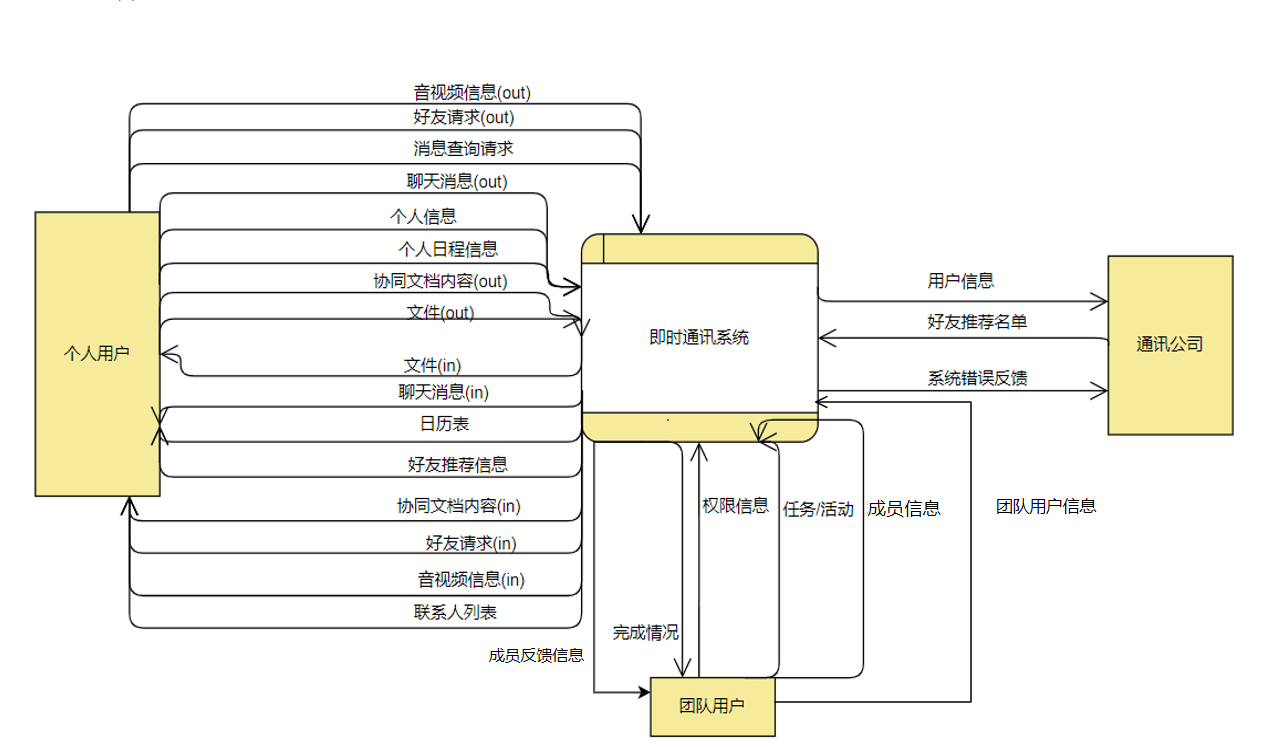
\includegraphics[scale = 0.55]{总体需求.png}\label{tab:classification}
            \caption{需求概念图}\label{fig:noted-figure}
        \end{figure}

\section{条件与限制}
\subsection{技术}
即时通讯系统的主要功能是提供现代工作场景下信息
交互,通知发布,团队组织、任务管理的平台解决方案。所依赖的的安卓、IOS、
Windows、Linux 操作系统,Intel 和智能移动端硬件平台,JAVA 开发语言和 Eclipse
开发环境都是成熟的开发生态圈,技术上可行。
\subsection{成本}
经济可行性上,本团队人力成本相对大型互联网企业偏低,场地使用学校实
验室不需要支付额外的费用,开发除了硬件消耗,服务器租用,软件维护的少量
费用以外,不存在其余开发费用。启动资金在个人承受范围以内,经营成本相对
低。通过广告、融资之后硬件和人力经济压力也会有所缓解, 因此经济上具有可
行性。
\subsection{法律}
即时通讯系统需要保障数据安全与用户隐私,具有法律上的责任。
本项目不侵犯任何其他工作的专利权和版权,具有法律可行性。

\chapter{总体设计}
%==================================================================
\section{软件描述}
    系统包括前台和后台两个部分。
\subsection{前台主要功能}
    向服务器发送请求,并接受服务器的响应,向用户展示服务器的返回结果。
    
    \begin{itemize}
        \item 用户可以进行账户注册,并使用已经注册的账户登录该系统。
        \item 用户可以与其他用户进行聊天。除了基本的文字聊天,用户还可以进行音视频聊天。此外,用户可以查看自己的聊天记录。
        \item 用户可以在群聊中发言。如果身份是管理员或群主,用户还可以对群聊进行管理。此外,不同的群聊情境还会提供不同的额外群聊功能。
        \item 用户可以对自己的通讯录进行管理:可以添加或删除好友,在添加好友时系统会进行个性化推荐;可以加入或退出群聊;可以将其他用户移入或移出黑名单。
        \item 用户可以对自己的Board进行管理,新建或修改日志;也可以浏览他人的Board,对他们的日志进行评论。
        \item 用户可以进行在线文档协作。
        \item 在接收到新的信息时,用户可以得到提醒。
        \item 用户在加入组织后,可以进行活动管理,自动修改所有参与者的日历。
        \item 用户可以查看并修改自己的日历。  
        \item 用户可以管理本地和云端的文件。
        \item 用户可以将账号与邮箱或设备进行绑定,以提高账户的安全性。
        \item 用户可以通过邮箱接口得知是否有新的邮件。
    \end{itemize}
    
\subsection{后台主要功能}
后台服务器接收用户发送的动作和请求,予以处理并进行响应。

服务器在接收到用户请求时,会在服务器的数据库中进行查询操作,并且进
行返回查询结果或者反馈提示信息,对于用户提交的数据(比如发布活动、修改日志等),也会存入到数据库中。对于发送的聊天信息,服务器会将其缓存到发送队列中。

%==================================================================
\section{处理流程}
    %--------------------------------------------------------------
    \subsection{总体流程}
        此处应当有一个图和对应的描述。
        \begin{figure}[ht]
            \centering
            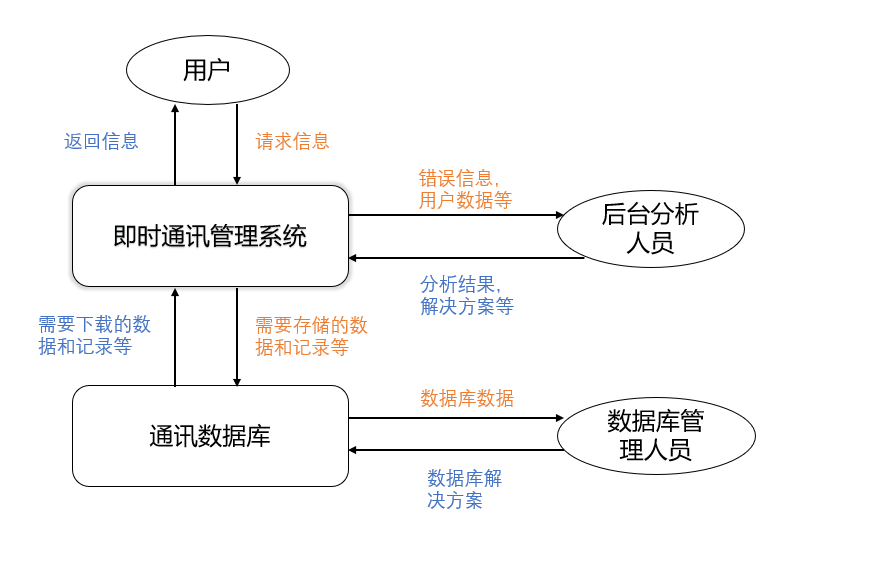
\includegraphics[scale = 0.75]{总体流程.png}\label{tab:classification}
            \caption{总体流程}\label{fig:noted-figure}
        \end{figure}
    %--------------------------------------------------------------
    \subsection{系统基本流程}
        此处应当有一个图和对应的描述。
    %--------------------------------------------------------------
    \subsection{客户端基本流程}
        这只是举个例子,如果没有客户端则不需要此节。
    %--------------------------------------------------------------
    \subsection{服务器端基本流程}
    服务器端流程如图\ref{fig:server_flow}所示。客户端1和2展示了一对一聊天和群聊的服务器处理过程;客户端4和5展示了音视频通讯的过程;
    客户端1与服务器间的箭头展示了查询的过程;客户端3与服务器间的箭头展示了更新的过程(许多功能都可以抽象为查询和更新,在后面会详细说明)。
    服务器使用SQL语句向数据库集群发送查询或更新请求,集群返回查询或更新的结果。
        \begin{figure}
            \centering
            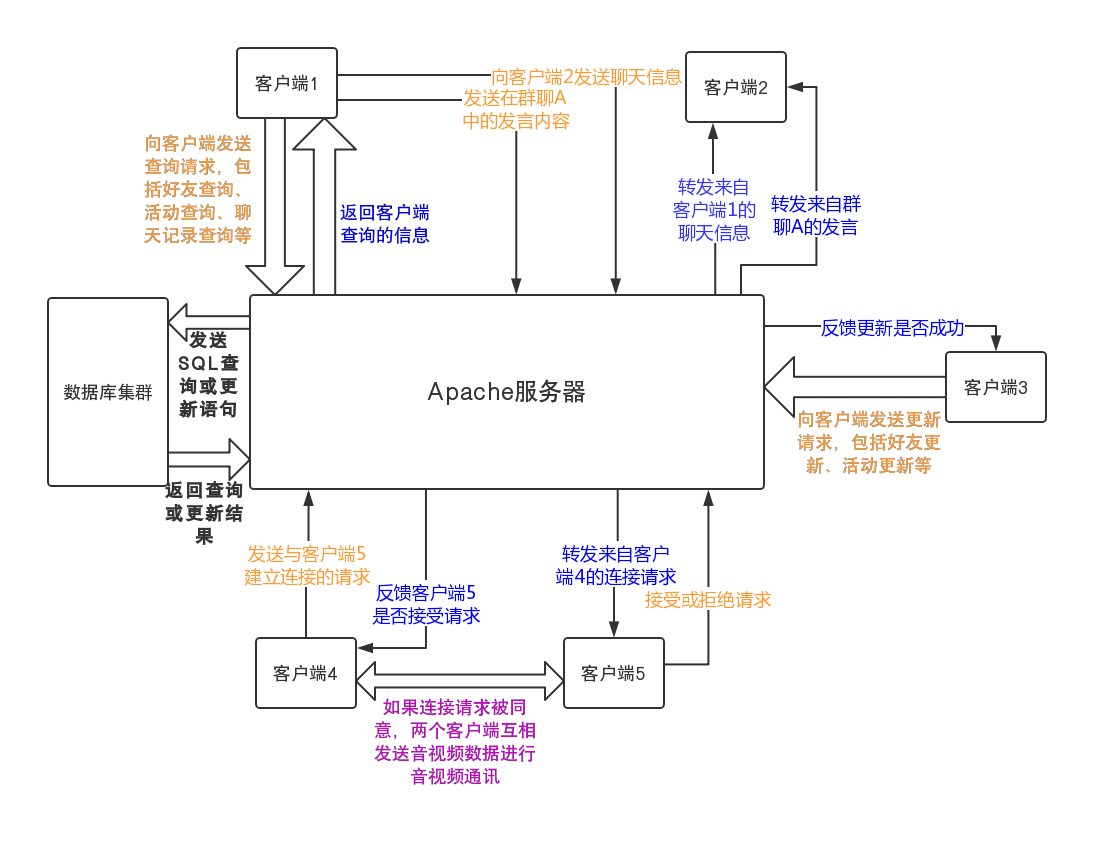
\includegraphics[scale=0.4]{OutlineDesign/figures/server_flow.png}
            \caption{服务器端流程}
            \label{fig:server_flow}
        \end{figure}
    %--------------------------------------------------------------
    \subsection{R.INTF.CALC.001: 一对一即时通讯功能·具体流程}
        已登录用户
    %--------------------------------------------------------------
%================ EXAMPLE ===================================================
% 已登录用户在购物车中提交请求交易的 POST 请求,提交的表单中指明了交易中包括的
% 所有商品、商家、付款信息、收货地址,输入输出处理系统接收到合法请求后,向商品信息
% 系统请求数据,收到数据以后验证是否正确,然后向订单系统发起生成新订单的请求,订单
% 系统负责更新商品信息系统、商家信息,通知商家接单,返回订单处理结果输入输出处理系
% 统,输入输出处理系统依照结果产生 HTML 页面,并返回给用户。
%================ EXAMPLE ===================================================
    \subsection{R.INTF.CALC.002: 多情境群聊功能·具体流程}
        %--------------------------------------------------------------
        \subsubsection{R.INTF.CALC.002.1: 群管理·具体流程}
        %--------------------------------------------------------------
        \subsubsection{R.INTF.CALC.002.2: 群聊天·具体流程}
        %--------------------------------------------------------------
        \subsubsection{R.INTF.CALC.002.3: 情境功能·具体流程}
        %--------------------------------------------------------------
    \subsection{R.INTF.CALC.003: 活动/任务发布与管理功能·具体流程}
    %--------------------------------------------------------------
    \subsection{R.INTF.CALC.004: 音视频通话 (会议) 功能·具体流程}
    %--------------------------------------------------------------
    \subsection{R.INTF.CALC.005: 通讯录功能·具体流程}
        %--------------------------------------------------------------
        \subsubsection{R.INTF.CALC.005.1: 好友管理·具体流程}
        %--------------------------------------------------------------
        \subsubsection{R.INTF.CALC.005.2: 群聊管理·具体流程}
        %--------------------------------------------------------------
        \subsubsection{R.INTF.CALC.005.3: 黑名单·具体流程}
        %--------------------------------------------------------------
    \subsection{R.INTF.CALC.006: 聊天记录功能·具体流程}
    %--------------------------------------------------------------
    \subsection{R.INTF.CALC.007: 消息提醒功能·具体流程}
    %--------------------------------------------------------------
    \subsection{R.INTF.CALC.008: Board(广场) 功能·具体流程}
    %--------------------------------------------------------------
    \subsection{R.INTF.CALC.009: 个性化好友推荐功能·具体流程}
    %--------------------------------------------------------------
    \subsection{R.INTF.CALC.010: 在线文档协作平台功能·具体流程}
    %--------------------------------------------------------------
    \subsection{R.INTF.CALC.011: 账号保护和隐私保护功能·具体流程}
    %--------------------------------------------------------------
    \subsection{R.INTF.CALC.012: 日历管理功能·具体流程}
    %--------------------------------------------------------------
    \subsection{R.INTF.CALC.013: 个人本地和云端文件管理功能·具体流程}
    %--------------------------------------------------------------
    \subsection{R.INTF.CALC.014: 邮箱接口功能·具体流程}
    %--------------------------------------------------------------
%==================================================================
\section{功能结构设计}
    %--------------------------------------------------------------
    \subsection{整体结构}
    
%============================== GUIDE ========================================
% 此处应当有一个图和对应的描述。系统如果像微内核那样,划分成核心模块和若干个子
% 系统,此处应当有图示及说明,然后后续几个节应当描述这几个子系统。如果系统像宏
% 内核,那应当说明有哪些紧密联系的模块,并在后续几个节内描述这些模块。
%============================== GUIDE ========================================
    \subsection{用户端结构}
%============================== GUIDE ========================================
% 此处应当有一个图和对应的描述。这只是举个例子。可能的内容包括用户端的具体模
% 块、耦合情况等。
%============================== GUIDE ========================================
    \subsection{服务器端结构}
%============================== GUIDE ========================================
% 此处应当有一个图和对应的描述。这只是举个例子。
%============================== GUIDE ========================================
    \subsection{后台数据库维护模块结构}
%============================== GUIDE ========================================
% 此处应当有一个图和对应的描述。这只是举个例子。
%============================== GUIDE ========================================
%==================================================================
\section{功能需求与程序代码的关系}
%============================== GUIDE ========================================
% [此处指的是不同的需求分配到哪些模块去实现。可按不同的端拆分此表]
%============================== GUIDE ========================================
    \begin{table}[htbp]
        \centering
        \small
        \caption{功能需求与程序代码的关系表} \label{tab:requirement-module}
            \begin{tabular}{|p{9em}|p{2.5em}|p{2.5em}|p{2.5em}|p{2.5em}|p{2.5em}|
                            p{2.5em}|p{2.5em}|p{2.5em}|}
            \hline %**********************************************************
            ·   & 用户信息管理模块      & 错误信息处理模块  & 云文件管理模块 
                & 文件管理模块          & 日历管理模块      & 团队管理模块      
                & 在线文档协作平台模块  & 通讯管理模块\\
            \hline %**********************************************************
            R.INTF.CALC.001: 一对一即时通讯功能
            %   & 用户信息管理模块      & 错误信息处理模块  & 云文件管理模块 
                & Y                     & Y                 & · 
            %   & 文件管理模块          & 日历管理模块      & 团队管理模块  
                & Y                     & ·                 & · 
            %   & 在线文档协作平台模块  & 通讯管理模块      \\
                & ·                     & Y                 \\
            \hline  %**********************************************************
            R.INTF.CALC.002: 多情境群聊功能
            %   & 用户信息管理模块      & 错误信息处理模块  & 云文件管理模块 
                & Y                     & Y                 & Y
            %   & 文件管理模块          & 日历管理模块      & 团队管理模块  
                & Y                     & ·                 & Y 
            %   & 在线文档协作平台模块  & 通讯管理模块      \\
                & ·                     & Y                 \\
            \hline %**********************************************************
            R.INTF.CALC.003: 活动/任务发布与管理功能
            %   & 用户信息管理模块      & 错误信息处理模块  & 云文件管理模块 
                & Y                     & Y                 & · 
            %   & 文件管理模块          & 日历管理模块      & 团队管理模块  
                & ·                     & Y                 & Y 
            %   & 在线文档协作平台模块  & 通讯管理模块      \\
                & ·                     & ·                 \\
            \hline %**********************************************************
            R.INTF.CALC.004: 音视频通话 (会议) 功能
            %   & 用户信息管理模块      & 错误信息处理模块  & 云文件管理模块 
                & Y                     & Y                 & · 
            %   & 文件管理模块          & 日历管理模块      & 团队管理模块  
                & ·                     & ·                 & · 
            %   & 在线文档协作平台模块  & 通讯管理模块      \\
                & ·                     & Y                 \\
            \hline %**********************************************************
            R.INTF.CALC.005: 通讯录功能
            %   & 用户信息管理模块      & 错误信息处理模块  & 云文件管理模块 
                & Y                     & Y                 & · 
            %   & 文件管理模块          & 日历管理模块      & 团队管理模块  
                & ·                     & ·                 & · 
            %   & 在线文档协作平台模块  & 通讯管理模块      \\
                & ·                     & ·                 \\
            \hline %**********************************************************
            R.INTF.CALC.006: 聊天记录功能
            %   & 用户信息管理模块      & 错误信息处理模块  & 云文件管理模块 
                & Y                     & Y                 & · 
            %   & 文件管理模块          & 日历管理模块      & 团队管理模块  
                & ·                     & ·                 & · 
            %   & 在线文档协作平台模块  & 通讯管理模块      \\
                & ·                     & Y                 \\
            \hline %**********************************************************
            R.INTF.CALC.007: 消息提醒功能
            %   & 用户信息管理模块      & 错误信息处理模块  & 云文件管理模块 
                & Y                     & Y                 & · 
            %   & 文件管理模块          & 日历管理模块      & 团队管理模块  
                & ·                     & Y                 & Y 
            %   & 在线文档协作平台模块  & 通讯管理模块      \\
                & ·                     & Y                 \\
            \hline %**********************************************************
            R.INTF.CALC.008: Board(广场)功能
            %   & 用户信息管理模块      & 错误信息处理模块  & 云文件管理模块 
                & Y                     & Y                 & · 
            %   & 文件管理模块          & 日历管理模块      & 团队管理模块  
                & ·                     & Y                 & · 
            %   & 在线文档协作平台模块  & 通讯管理模块      \\
                & ·                     & ·                 \\
            \hline %**********************************************************
            R.INTF.CALC.009: 个性化好友推荐功能
            %   & 用户信息管理模块      & 错误信息处理模块  & 云文件管理模块 
                & Y                     & Y                 & · 
            %   & 文件管理模块          & 日历管理模块      & 团队管理模块  
                & ·                     & ·                 & · 
            %   & 在线文档协作平台模块  & 通讯管理模块      \\
                & ·                     & Y                 \\
            \hline %**********************************************************
            R.INTF.CALC.010: 在线文档协作平台功能
            %   & 用户信息管理模块      & 错误信息处理模块  & 云文件管理模块 
                & Y                     & Y                 & Y 
            %   & 文件管理模块          & 日历管理模块      & 团队管理模块  
                & ·                     & ·                 & Y 
            %   & 在线文档协作平台模块  & 通讯管理模块      \\
                & Y                     & ·                 \\
            \hline %**********************************************************
            R.INTF.CALC.011: 账号保护和隐私保护功能
            %   & 用户信息管理模块      & 错误信息处理模块  & 云文件管理模块 
                & Y                     & Y                 & · 
            %   & 文件管理模块          & 日历管理模块      & 团队管理模块  
                & ·                     & ·                 & · 
            %   & 在线文档协作平台模块  & 通讯管理模块      \\
                & ·                     & ·                 \\
            \hline %**********************************************************
            R.INTF.CALC.012: 日历管理功能
            %   & 用户信息管理模块      & 错误信息处理模块  & 云文件管理模块 
                & Y                     & Y                 & · 
            %   & 文件管理模块          & 日历管理模块      & 团队管理模块  
                & ·                     & Y                 & Y 
            %   & 在线文档协作平台模块  & 通讯管理模块      \\
                & ·                     & ·                 \\
            \hline %**********************************************************
            R.INTF.CALC.013: 个人本地和云端文件管理功能
            %   & 用户信息管理模块      & 错误信息处理模块  & 云文件管理模块 
                & Y                     & Y                 & Y 
            %   & 文件管理模块          & 日历管理模块      & 团队管理模块  
                & Y                     & ·                 & · 
            %   & 在线文档协作平台模块  & 通讯管理模块      \\
                & Y                     & Y                 \\
            \hline %**********************************************************
            R.INTF.CALC.014: 邮箱接口功能
            %   & 用户信息管理模块      & 错误信息处理模块  & 云文件管理模块 
                & Y                     & Y                 & · 
            %   & 文件管理模块          & 日历管理模块      & 团队管理模块  
                & ·                     & ·                 & · 
            %   & 在线文档协作平台模块  & 通讯管理模块      \\
                & ·                     & ·                 \\
            \hline %**********************************************************
            \end{tabular}
        \note{本表体现了各项功能需求的实现与各个程序模块的分配关系}
    \end{table}
%==================================================================
\chapter{接口设计}
%====================================================================================
\section{外部接口}
%====================================================================================
% 比如说需要用到支付宝等外部支付系统,接口应当如何封装。
%====================================================================================
JavaMail是由Sun发布的用来处理email的API,它是Java EE的一部分。我们调用该接口查询和发送邮件。

\section{内部接口}
\subsection{用户信息管理模块}
\begin{lstlisting}[language=Java, caption=用户信息管理模块接口]
public class UserInfoManager{
    public static void uploadUser(User user){
        //将用户信息上传到服务器
    }
    public static User downloadUser(String userID){
        //从服务器下载对应ID的用户信息
    }
    public static User[] getRecommandedFriends(){
        //向服务器获取个性化的推荐好友
    }
    public static void sendFriendRequest(User user){
        //发送好友请求
    }
    public static SystemMessage[] receiveFriendRequest(){
        //获取发送给自己的好友请求
    }
    public static void responseFriendRequest(
        SystemMessage request,boolean accept){
        //对好友请求进行回复
    }
}

\end{lstlisting}




\subsection{通讯管理模块}
{\color{red}

\begin{lstlisting}[language=Java, caption=通讯管理模块接口]
public class CommunicationManager{
    public static void sendMessage(Message message){
        //发送信息
    }
    public static Message receiveMessage(){
        //接收信息(阻塞)
    }
    public static boolean sendRadioConnectionRequest(
        User user,int type){
        //发送音视频连接请求(阻塞+超时机制)
    }
    public static Connection 
        receiveRadioConnectionRequest(){
        //获取并回复发送给自己的音视频连接请求
    }
    public static void sendRadio(Connection connection,
        byte[] data){
        //发送音视频数据
    }
    public static byte[] receiveRadio(
        Connection connection){
        //接收发送给自己的音视频数据
    }
    public static void uploadMessage(Message message){
        //上传聊天信息
    }
    public static Message[] downloadMessage(
        User user,Date date){
        //下载与指定对象在指定时间的聊天记录(null不进行指定)
    }
    
    public static void publishIssue(Issue issue){
        //发布一个issue
    }
    
    public static void answerIssue(Issue issue, Answer answer){
        //回答指定的issue
    }
    
    public static void closeIssue(Issue issue){
        //关闭指定的Issue
    }
    
    
}
\end{lstlisting}
}
\subsection{文件管理模块}
\begin{lstlisting}[language=Java, caption=文件管理模块接口]
public class FileManager{
    public static void saveFile(File file,String path){
        //保存文件
    }
    public static File loadFile(String path){
        //加载指定文件
    }
    public static String[] searchFile(String name){
        //查询指定文件
    }
    public static Message sendFile(User user,File file){
        //向指定用户发送文件,文件信息存放在返回的Message中。
        //这个Message将被发送给对方,对方可以使用这个Message接收文件
    }
    public static File receiveFile(Message message){
        //使用存放有文件信息的Message接收文件
    }

}
\end{lstlisting}

\subsection{云文件管理模块}
\begin{lstlisting}[language=Java, caption=云文件管理模块接口]
public class CloudFileManager{
    public static String defaultURL;
    public static void uploadFile(File file,String url){
        //上传云文件
    }
    public static File downloadFile(String url){
        //下载云文件
    }
    public static String[] searchFile(String name){
        //查询指定的云文件
    }
    public static String getFileInfo(String url){
        //得到指定url对应的文件信息
    }
}
\end{lstlisting}

\subsection{团队管理模块}
\begin{lstlisting}[language=Java, caption=团队管理模块接口]
public class GroupManager{
    public static void uploadFile(Group group,File file){
        //上传群文件
    }
    public static File downloadFile(Group group,
        String name){
        //下载群文件
    }
    public static Group createGroup(User user,String name){
        //创建群聊
    }
    public static Group getGroup(String groupID){
        //得到对应ID的群聊
    }
    public static void disbandGroup(Group group){
        //解散群聊
    }
    public static void updateGroupInfo(Group group,
        int type,User user){
        //对群管理信息进行更新,包括增减群成员和改变群成员权限
    }
    public static void publishTask(Group group,Task task){
        //发布任务
    }
    public static void updateTask(Group group,Task task){
        //更新任务
    }
}
\end{lstlisting}

\subsection{日历管理模块}
\begin{lstlisting}[language=Java, caption=日历管理模块接口]
public class CalanderManager{
    public static Activity[][] calanderBuffer;
    public static Activity[] downloadActivities(){
        //下载活动项
    }
    public static void uploadActivity(Activity activity){
        //上传活动项
    }
    public static void deleteActivity(Activity activity){
        //删除活动项
    }
    public static void addActivity(Activity activity){
        //新增活动项
    }
    public static void getActivities(Date date,int length){
        //获取某一段时间的所有活动,写入calanderBuffer
    }
}
\end{lstlisting}

\subsection{共享文档管理模块}
\begin{lstlisting}[language=Java, caption=共享文档管理模块接口]
public class DocumentCooperationManager{
    public static String createDocument(File file){
        //创建共享文档,返回URL
    }
    public static File openDocument(String url){
        //使用URL打开共享文档
    }
    public static void sendUpdate(String url,Update update){
        //发送更改
    }
    public static Update receiveUpdate(){
        //接收更改
    }
    public static File applyUpdate(File file,Update update){
        //应用更改
    }
}
\end{lstlisting}

\subsection{错误管理模块}
\begin{lstlisting}[language=Java, caption=错误管理模块接口]
public class ErrorManager{
    public static void reportError(Exception ex){
        //向服务器报告错误
    }
}
\end{lstlisting}


{\color{red}

\subsection{\color{red}爬虫模块}
\begin{lstlisting}[language=Java, caption=爬虫模块接口]
public class CrawlerManager{
    public static String fetch(URL url){
        //爬取网页,并返回重要信息
    } 
    public static String[] analyse(String s){
        //解析网页信息
    }
}
\end{lstlisting}

\subsection{\color{red}信息调研模块}
\begin{lstlisting}[language=Java, caption=信息调研模块接口]
public class SurveyManager{
    public static Survey downloadSurvey(){
        //下载问卷
    }
    public static void uploadSurvey(Survey survey){
        //上传问卷
    }
    public static void updateSurvey(Survey survey){
        //更新问卷
    }
}
\end{lstlisting}


\subsection{\color{red}流程审批模块}
\begin{lstlisting}[language=Java, caption=流程模块接口]
public class ApprovalManager{
    public static Approval downloadApproval(){
        //下载审批
    }
    public static void uploadApproval(Approval approval){
        //上传审批
    }
    public static void acceptApproval(Approval approval,String opinion){
        //批准审批
    }
    public static void refuseApproval(Approval approval,String opinion){
        //不批准审批
    }
}
\end{lstlisting}


}

\chapter{数据结构设计}
%=================================================================================
    \section{逻辑结构设计}
    %-----------------------------------------------------------------------------

        %================================ GUIDE ==================================
        % 讲述本系统内需要什么数据结构。这指的是程序运行过程中维护的数据结构。
        % 只是举个例子,此处应和3.3一致。
        %================================ GUIDE ==================================
    %-----------------------------------------------------------------------------
        \subsection{客户端数据结构}
        
    %-----------------------------------------------------------------------------

        
    %-----------------------------------------------------------------------------
\subsubsection{数据结构1:User\_client}
该数据结构定义了用户的基本属性。
\begin{lstlisting}[language=Java, caption=User定义]
public class User{
    private String ID;//用户ID,唯一
    private String name;//昵称,不唯一
    private String sex="Male";//性别,默认男性
    private Date birthday;//用户的出生日期,可以为空
    private Time createTime;//账户创建时间
    private String address;//用户地址,可以为空
    private String email;//用户绑定的邮箱,可以为空
    public User(String ID){

    }
    public User(String ID,String name,String sex,
        Date birthday,String address,String email){

    }
    public String getID(){

    }
    public String getName(){

    }
    public void setName(String name){

    }
    public String getSex(){

    }
    public void setSex(String sex){

    }
    public Date getBirthday(){

    }
    public void setBirthday(Date birthday){

    }
    public int getAge(){

    }
    public Time getCreateTime(){

    }
    public void setCreateTime(Time createTime){

    }
    public String getAddress(){

    }
    public void setAddress(String address){

    }
    public String getEmail(){

    }
    public void setEmail(String email){

    }
}
\end{lstlisting}

\subsubsection{数据结构2:Message\_client}
该数据结构定义了一对一聊天时发送的信息,所有属性都是不可修改的。此外,在发送文件时,该数据结构也会被使用,用于声明文件的一些基本信息(使用message域)。
\begin{lstlisting}[language=Java, caption=Message定义]
public class Message{
    private User sender,receiver;//该信息的发送方和接收方
    private String message;//信息内容
    private Time sendtime;//发送时间
    public Message(User sender,User receiver,String message,
        Time sendtime){

    }
    public User getSender(){

    }
    public User getReceiver(){

    }
    public String getMessage(){
        
    }
    public Time getSendtime(){

    }
}
\end{lstlisting}
    
\subsubsection{数据结构3:GroupMessage\_client}
该数据结构定义了群聊时发送的信息,继承自Message类。同样,所有属性都是不可修改的。
\begin{lstlisting}[language=Java, caption=GroupMessage定义]
public class GroupMessage extends Message{
    private Group group;//所属的群聊
    public GroupMessage(Group group,User sender,
        User receiver, String message,Time sendtime){

    }
    public Group getGroup(){

    }
}
\end{lstlisting}

\subsubsection{数据结构4:Group\_client}
该数据结构定义了群聊的基本属性。
\begin{lstlisting}[language=Java, caption=Group定义]
public class Group{
    private String ID;//群ID,唯一
    private String name;//群名称,不唯一
    private User master;//群主
    private User[] managerList;//管理员列表
    private User[] memberList;//群成员列表
    private Scene scene; //场景
    public Group(String ID,User master){

    }
    public String getID(){

    }
    public String getName(){

    }
    public void setName(String name){

    }
    public User getMaster(){

    }
    public User[] getManagerList(){

    }
    public User[] getMemberList(){

    }
    public void appointManager(User user){
    //任命管理员
    }
    public void dismissManager(User user){
    //解除管理员职务
    }
    public void addMember(User user){
    //增加群成员
    }
    public void deleteMember(User user){
    //删除群成员
    }
    public Scene getScene(){

    }
    public void setScene(Scene scene){
        
    }
}
\end{lstlisting}

\subsubsection{数据结构5:Friend\_client}
该数据结构定义了通讯录中好友的基本属性。通讯录可以对好友分组管理,这是通过tag实现的,具有相同tag的用户被认为是一个组。
\begin{lstlisting}[language=Java, caption=Friend定义]
public class Friend{
    private User user;//用户
    private String tag;//分组标记,内容是组名
    private String remark;//备注名
    public Friend(User user,String tag,String remark){

    }
    public User getUser(){

    }
    public String getTag(){

    }
    public void setTag(String tag){

    }
    public String getRemark(){

    }
    public void setRemark(String remark){

    }
}
\end{lstlisting}

\subsubsection{数据结构6:AddressBook\_client}
该数据结构定义了通讯录,包括好友列表,群聊列表和黑名单。
\begin{lstlisting}[language=Java, caption=AddressBook定义]
public class AddressBook{
    private Friend[] friendList;//好友列表
    private User[] blackList;//黑名单
    private Group[] groupList;//群聊列表
    public AddressBook(){

    }
    public Friend[] getFriendList(){

    }
    public User[] getBlackList(){

    }
    public Group[] getGroupList(){

    }
    public void addFriend(User user){

    }
    public void addFriend(Friend friend){

    }
    public void deleteFriend(Friend friend){
        
    }
    public void addBlack(User user){

    }
    public void deleteBlack(User user){

    }
    public void addGroup(Group group){

    }
    public void deleteGroup(Group group){

    }
    public Friend[] findFriendByTag(String tag){
        //查找某一组的所有好友
    }
}
\end{lstlisting}

\subsubsection{数据结构7:Task\_client}
该数据结构定义了任务的基本属性,它将在活动/任务发布与管理功能中应用。
\begin{lstlisting}[language=Java, caption=Task定义]
public class Task{
    private User organizer;//组织者
    private User[] participants;//参与者列表
    private String address;//任务地点
    private Time time;//任务时间
    private String content;//任务内容
    public Task(){

    }
    public User getOrganizer(){

    }
    public User[] getParticipants(){

    }
    public void setParticipants(User[] participants){

    }
    public void addParticipant(User participant){

    }
    public void deleteParticipant(User participant){

    }
    public String getAddress(){

    }
    public void setAddress(String address){

    }
    public Time getTime(){

    }
    public void setTime(Time time){

    }
    public String getContent(){

    }
    public void setContent(){

    }
}
\end{lstlisting}

\subsubsection{数据结构8:Activity\_client}
该数据结构定义了活动项的基本属性,将被用于日历应用。
\begin{lstlisting}[language=Java, caption=Activity定义]
public class Activity{
    private Date date;//活动日期
    private Time time;//活动具体时间
    private String content;//活动内容
    public Activity(Date date, Time time, String content){

    }
    public Date getDate(){

    }
    public void setDate(Date date){

    }
    public Time getTime(){

    }
    public void setTime(){

    }
    public String getContent(){

    }
    public void setContent(String content){
        
    }
}
\end{lstlisting}

\subsubsection{数据结构9:SystemMessage\_client}
该数据结构定义了系统消息,继承自Message类。
\begin{lstlisting}[language=Java, caption=SystemMessage定义]
public class SystemMessage extends Message{
    private int type; //系统消息类型
    public SystemMessage(User sender,User reciver,
        String message,Time sendtime,int type){

    } 
    public int setType(){

    }
}
\end{lstlisting}

\subsubsection{数据结构10:Update\_client}
该数据结构定义了对共享文档的原子更改,所有属性都是不可更改的。
\begin{lstlisting}[language=Java, caption=Update定义]
public class Update{
    private int pos;//修改位置
    private int type;//修改类型(增、删、改)
    private int length;//修改长度
    private String updateText;//修改后的内容
    private String url;//修改的文件的URL
    public Update(int pos,int type,int length,
        String updateText,String url){

    }
    public int getPos(){

    }
    public int getType(){

    }
    public int getLength(){

    }
    public Stirng getUpdateText(){

    }
    public String getURL(){

    }
}
\end{lstlisting}

{\color{red}

\subsubsection{数据结构11:Survey\_client}
该数据结构定义了调查问卷的基本属性,以及问题的属性(包括选择题和问答题),将被用于信息调研模块。
\begin{lstlisting}[language=Java, caption=Survey定义]

public class Survey{
    private String title;//标题
    private String introduction;//简介
    private ArrayList<Question> questions;//问题列表
    private int mode;//模式
    private ArrayList<User> respondents;//允许填写问卷的用户列表,null代表所有人

    public String getTitle() {
        return title;
    }
    public void setTitle(String title) {
        this.title = title;
    }
    public String getIntroduction() {
        return introduction;
    }
    public void setIntroduction(String introduction) {
        this.introduction = introduction;
    }
    public ArrayList<Question> getQuestions() {
        return questions;
    }
    public void setQuestions(ArrayList<Question> questions) {
        this.questions = questions;
    }

    public int getMode() {
        return mode;
    }

    public void setMode(int mode) {
        this.mode = mode;
    }

    public ArrayList<User> getRespondents() {
        return respondents;
    }

    public void setRespondents(ArrayList<User> respondents) {
        this.respondents = respondents;
    }   
}


abstract class Question{
    String description;
}

class MultipleChoiceQuestion extends Question{
    String[] items;//选项
    ArrayList<User>[] choices; //选择每一个选项的用户列表

    public MultipleChoiceQuestion(String[] items) {

    }
    public void insertChoice(User user,int item){
        
    }   
}
class AnswerQuestion extends Question{
    HashMap<User,String> answerMap;//每一个用户和他的答案

    public AnswerQuestion() {
    }
    public void insertAnswer(User user,String answer){
        
    }
}
\end{lstlisting}

\subsubsection{数据结构12:Approval\_client}
该数据结构定义了审批流程的基本属性,用于审批模块。
\begin{lstlisting}[language=Java, caption=Approval定义]
public class Approval {
    private String content;//申请内容
    private File[] annex;//附件列表
    private int mode;//模式
    private ArrayList<User> managers;//有序的经办人列表
    private ArrayList<String> opinions;//每一个经办人的意见
    private ArrayList<Boolean> agreed;//每一个经办人是否批准

    public String getContent() {
        return content;
    }

    public void setContent(String content) {
        this.content = content;
    }

    public File[] getAnnex() {
        return annex;
    }

    public void setAnnex(File[] annex) {
        this.annex = annex;
    }

    public int getMode() {
        return mode;
    }

    public void setMode(int mode) {
        this.mode = mode;
    }

    public ArrayList<User> getManagers() {
        return managers;
    }

    public void setManagers(ArrayList<User> managers) {
        this.managers = managers;
    }

    public ArrayList<String> getOpinions() {
        return opinions;
    }

    public void setOpinions(ArrayList<String> opinions) {
        this.opinions = opinions;
    }

    public ArrayList<Boolean> getAgreed() {
        return agreed;
    }

    public void setAgreed(ArrayList<Boolean> agreed) {
        this.agreed = agreed;
    }
    
}
\end{lstlisting}

\subsubsection{数据结构13:Issue\_client}
该数据结构定义了Issue的基本属性,以及被其使用的回答类的属性。

\begin{lstlisting}[language=Java, caption=Issue定义]
public class Issue {
    private String question;//问题内容
    private User creater;//问题发布者
    private Time time;//发布时间
    private boolean closed;//问题是否关闭
    private ArrayList<Answer> answers;//回答列表

    public Issue() {
    }
    
    public String getQuestion() {
        return question;
    }

    public void setQuestion(String question) {
        this.question = question;
    }

    public User getCreater() {
        return creater;
    }

    public void setCreater(User creater) {
        this.creater = creater;
    }

    public boolean isClosed() {
        return closed;
    }

    public void setClosed(boolean closed) {
        this.closed = closed;
    }

    public ArrayList<Answer> getAnswers() {
        return answers;
    }

    public void setAnswers(ArrayList<Answer> answers) {
        this.answers = answers;
    }

    public Time getTime() {
        return time;
    }

    public void setTime(Time time) {
        this.time = time;
    }
    
}

class Answer{
    private String content;//回答内容
    private User author;//回答作者
    private Time time;//发布时间
    private boolean recommended;//是否被issue发布者置顶

    public Answer(String content, User author, Time time) {

    }
    
    public String getContent(){
    
    }
    
    public void setContent(String content){
    
    }
    
    public boolean getRecommend(){
        
    }
    public void setRecommend(boolean b){
        
    }
}
\end{lstlisting}


}





\subsection{服务器端数据结构}
%--------
\subsubsection{数据结构1:User\_server}
该数据结构定义了用户的基本属性。
\begin{lstlisting}[language=Java, caption=User定义]
public class User{
    private String ID;//用户ID,唯一
    private String name;//昵称,不唯一
    private String sex="Male";//性别,默认男性
    private Date birthday;//用户的出生日期,可以为空
    private Time createTime;//账户创建时间
    private String address;//用户地址,可以为空
    private String email;//用户绑定的邮箱,可以为空
}
\end{lstlisting}

\subsubsection{数据结构2:Message\_server}
该数据结构定义了一对一聊天时发送的信息,所有属性都是不可修改的。此外,在发送文件时,该数据结构也会被使用,用于声明文件的一些基本信息(使用message域)。
\begin{lstlisting}[language=Java, caption=Message定义]
public class Message{
    private User sender,receiver;//该信息的发送方和接收方
    private String message;//信息内容
    private Time sendtime;//发送时间
}
\end{lstlisting}

\subsubsection{数据结构3:GroupMessage\_server}
该数据结构定义了群聊时发送的信息,继承自Message类。同样,所有属性都是不可修改的。
\begin{lstlisting}[language=Java, caption=GroupMessage定义]
public class GroupMessage extends Message{
    private Group group;//所属的群聊
}
\end{lstlisting}

\subsubsection{数据结构4:Group\_server}
该数据结构定义了群聊的基本属性。
\begin{lstlisting}[language=Java, caption=Group定义]
public class Group{
    private String ID;//群ID,唯一
    private String name;//群名称,不唯一
    private User master;//群主
    private User[] managerList;//管理员列表
    private User[] memberList;//群成员列表
    private Scene scene; //场景
}
\end{lstlisting}


\subsubsection{数据结构5:Friend\_server}
该数据结构定义了通讯录中好友的基本属性。通讯录可以对好友分组管理,这是通过tag实现的,具有相同tag的用户被认为是一个组。
\begin{lstlisting}[language=Java, caption=Friend定义]
public class Friend{
    private User user;//用户
    private String tag;//分组标记,内容是组名
    private String remark;//备注名
}
\end{lstlisting}


\subsubsection{数据结构6:AddressBook\_server}
该数据结构定义了通讯录,包括好友列表,群聊列表和黑名单。
\begin{lstlisting}[language=Java, caption=AddressBook定义]
public class AddressBook{
    private Friend[] friendList;//好友列表
    private User[] blackList;//黑名单
    private Group[] groupList;//群聊列表
}
\end{lstlisting}

\subsubsection{数据结构7:Task\_server}
该数据结构定义了任务的基本属性,它将在活动/任务发布与管理功能中应用。
\begin{lstlisting}[language=Java, caption=Task定义]
public class Task{
    private User organizer;//组织者
    private User[] participants;//参与者列表
    private String address;//任务地点
    private Time time;//任务时间
    private String content;//任务内容
}
\end{lstlisting}

\subsubsection{数据结构8:Activity\_server}
该数据结构定义了活动项的基本属性,将被用于日历应用。
\begin{lstlisting}[language=Java, caption=Activity定义]
public class Activity{
    private Date date;//活动日期
    private Time time;//活动具体时间
    private String content;//活动内容
}
\end{lstlisting}

\subsubsection{数据结构9:SystemMessage\_server}
该数据结构定义了系统消息,继承自Message类。
\begin{lstlisting}[language=Java, caption=SystemMessage定义]
public class SystemMessage extends Message{
    private int type; //系统消息类型
}
\end{lstlisting}

\subsubsection{数据结构10:Error\_server}
该数据结构定义了报错的结构体。
\begin{lstlisting}[language=Java, caption=Error定义]
public class SystemMessage extends Message{
    private int position; //出错位置
    private int type; //错误类型
    private Date date; //出错日期
    private Time time; //出错时间
}
\end{lstlisting}


{\color{red}

\subsubsection{数据结构11:Survey\_server}
该数据结构定义了调查问卷的基本属性,以及问题的属性(包括选择题和问答题),将被用于信息调研模块。
\begin{lstlisting}[language=Java, caption=Survey定义]

public class Survey{
    private String title;//标题
    private String introduction;//简介
    private ArrayList<Question> questions;//问题列表
    private int mode;//模式
    private ArrayList<User>  
}


abstract class Question{
    String description;
}

class MultipleChoiceQuestion extends Question{
    String[] items;//选项
    ArrayList<User>[] choices; //选择每一个选项的用户列表
}
class AnswerQuestion extends Question{
    HashMap<User,String> answerMap;//每一个用户和他的答案
}
\end{lstlisting}

\subsubsection{数据结构12:Approval\_server}
该数据结构定义了审批流程的基本属性,用于审批模块。
\begin{lstlisting}[language=Java, caption=Approval定义]
public class Approval {
    private String content;//申请内容
    private File[] annex;//附件列表
    private int mode;//模式
    private ArrayList<User> managers;//有序的经办人列表
    private ArrayList<String> opinions;//每一个经办人的意见
    private ArrayList<Boolean> agreed;//每一个经办人是否批准
}
\end{lstlisting}

\subsubsection{数据结构13:Issue\_server}
该数据结构定义了Issue的基本属性,以及被其使用的回答类的属性。

\begin{lstlisting}[language=Java, caption=Issue定义]
public class Issue {
    private String question;//问题内容
    private User creater;//问题发布者
    private Time time;//发布时间
    private boolean closed;//问题是否关闭
    private ArrayList<Answer> answers;//回答列表
}
class Answer{
    private String content;//回答内容
    private User author;//回答作者
    private Time time;//发布时间
    private boolean recommended;//是否被issue发布者置顶
}
\end{lstlisting}
}




\subsubsection{数据结构14:UserInfoManagement\_server}

\begin{lstlisting}[language=Java, caption=用户信息管理类]
public class UserInfoManagement{
    private static User[] Users;//存储所有的用户
    private static User[] OnlineUsers; //存储所有的在线用户
    
    public static void registerUser(User_server user){
        //用户注册
    }
    public static int selectUser(User_server user){
        //在Users列表中查询用户对应项
    }
    public static User_server[] recommendUser(User_server
    user){
        //推荐好友列表
    }
    public static AddressBook(
    
 User_server user){
        //查找某个user的联系人列表
    }   pserver(public static void deleteUser(User_server 
    user){
        //删除用户
    }
    public static void UpdateUser(int UserID){
        //更新Users列表中的User信息
        //(例如绑定邮箱后需更新Users列表中对应user的email项)
    }
    public static void upLoad(User_server user){
        //向数据库上传
    }
    public static User[] downLoad(User_server user){
        //从数据库下载用户信息,并打包为User结构体
    }
\end{lstlisting}

%--------
\subsubsection{数据结构15:CommunicationManagement\_server}
%--------
\begin{lstlisting}[language=Java, caption=通讯管理类]
public class CommunicationManagement{
    private static Message[] messageBuffer; 
    //存储待转发的消息队列
    
    public static Message_server Receive(Message_server
    
    message_received){
        //接收消息
    }
    public static void Send(Message_server message_send){
        //发送消息
    }
    public static void Transfer(User_server sender, 
    User\_server Receiver){
        //转发消息
    )
    public static void upLoad(Message_server message){
        //向数据库上传聊天记录
    }
    public static Message_server downLoad(Message_server 
    message){
        //从数据库下载聊天记录,并打包为Message类
    }
}
\end{lstlisting}
%--------
\subsubsection{数据结构16:CommunicationManagement\_server}
%--------
\begin{lstlisting}[language=Java, caption=文件管理类]
public class FileManagement{
    private static Message_server[]  FileRecord; 
    //记录所有的文件信息及其存储地址
    
    public static int selectRecord(Message_server record){
        //查询文件记录在FileRecord中的对应项
    }
    
    public static Message_server ReceiveFileRecord(){
        //接收文件记录(其为Message的一种类型,记录了发送者,
        接收者,存储地址等信息)
    }
    public static File ReceiveFile(int FileID){
        //接收文件, 并将其绑定到对应的文件记录
    }
    public static void SendFileRecord(Message_server 
    filerecord){
        //发送文件记录(其为Message的一种类型,记录了发送者,
        接收者,存储地址等信息)
    }
    public static void SendFile(Message_server filerecord,
    File file){
        //发送文件
    }
    public static void Transfer(Message_server filerecord,
    File file){
        //转发文件
    }
    public static void upLoad(Message_server record, 
    File file){
        //向数据库上传文件
    }
    public static File downLoad(Message_server record){
        //根据文件记录中的地址,从数据库下载文件
    }
    
}
\end{lstlisting}
%--------
\subsubsection{数据结构17:CalendarManagement\_server}
%--------
\begin{lstlisting}[language=Java, caption=日历管理类]
public class CalendarManagement{
    public static void Activity_server[][] calendarBuffer;
    
    //存储需要修改的日历
    
    public static int[] selectCalendar(Activity_server
    activity){
        //查找日历缓存表中的对应日历项
    }
    public static void addActivity(int[] calendarID, 
    Activity_server activity){
        //向单个或多个日历中添加活动
    }
    public static void deleteActivity(int[] calendarID, 
    Activity_server activity){
        //向单个或多个日历中删除活动
    }
    public static void updateActivity(int [] calendarID, 
    Activity_server activity){
        //向单个或多个日历中更新活动
    }
    public static void upLoad(Activity_server
    [] Calendar){
        //向数据库上传日历
    }
    public static Activity_server[] downLoad(
    Activity_server[] Calendar){
        //从数据库下载日历
    }
    
}
\end{lstlisting}
%--------
\subsubsection{数据结构18:GroupManagement\_server}
%--------
\begin{lstlisting}[language=Java, caption=团队管理类]
public static class GroupManagement{
    public static Group_server[] Groups;
    
    public static int selectGroup(Group_server group){
        //在群组管理列表中寻找对应项
    }
    public static void Assign_Task(Task_server[] task){
        //向组员发布任务
    }
    public static void setAuthority(Group_server group){
        //设置群组中用户的权限
    }
    public static void reflect(SystemMessage_server 
    message){
        //根据组员的反馈信息调整任务
    }
    public static void upLoad(Group_server[] group){
        //向数据库上传团队信息
    }
    public static Group_server[] downLoad(Group_server[] 
    group){
        //从数据库下载团队信息
    }
}
\end{lstlisting}
%--------
\subsubsection{数据结构19:CoopeartionManagement\_server}
%--------
\begin{lstlisting}[language=Java, caption=在线协作类]
public static class CoopeartionManagement{
    public static File[] fileBuffer;//协作文档缓冲池
    
    public static int selectFile(File file){
        //查找文件对应的缓冲池的项
    }
    public static void sendFile(File file){
        //向成员发送最新的文档
    }
    public static File receiveContent(){
        //接收修改的内容
    }
    public static File mergeFile(File file){
        //将对文件的增删改合并到当前文档中
    }
    public static void upLoad(File){
        //向数据库上传协作文档
    }
    public static File downLoad(File){
        //从数据库下载协作文档
    }
    
} 
\end{lstlisting}
%--------
\subsubsection{数据结构20:ErrorManagement\_server}
\begin{lstlisting}[language=Java, caption=在线协作类]
public static class ErrorManagement{

    public static Error receiveError(){
        //接收Error
    }
    public static void handleError(){
        //处理能够解决的error
    }
    public static void feedback(Error error){
        //将无法解决的Error反馈给公司
    }

} 
\end{lstlisting}




    %-----------------------------------------------------------------------------
    \section{物理结构设计}
    %-----------------------------------------------------------------------------
        各数据结构无特殊物理结构要求。
    %-----------------------------------------------------------------------------
    \section{数据结构与程序模块的关系}
    %================================ GUIDE ======================================
    % [此处指的是不同的数据结构分配到哪些模块去实现。可按不同的端拆分此表]
    %================================ GUIDE ======================================
{\color{red}
        \begin{table}[htbp]
            \centering
            \caption{数据结构与程序代码的关系表}
            \label{tab:datastructure-module}
            \begin{tabular}{|p{6.3em}|p{2em}|p{2em}|p{2em}|p{2em}|p{2em}|
                            p{2em}|p{2em}|p{2em}|p{2em}|p{2em}|p{2em}|}
                \hline %**********************************************************
            ·   & 用户信息管理模块      & 错误信息处理模块  & 云文件管理模块 
                & 文件管理模块          & 日历管理模块      & 团队管理模块      
                & 在线文档协作平台模块  & 通讯管理模块      &
                爬虫模块
                & 流程审批模块          & 信息调研模块
                \\
                \hline
                User                & Y   & Y     & · 
                                    & .   & .     & Y
                                    & .   & Y     & Y
                                    & Y   & Y     \\
                \hline
                Message             & .   & Y     & Y 
                                    & Y   & .     & .
                                    & .   & Y     & .
                                    & .   & .     \\
                \hline
                GrouopMessage       & .   & Y     & Y 
                                    & Y   & .     & Y
                                    & .   & Y     & .
                                    & .   & .     \\
                \hline
                Group               & .   & Y     & . 
                                    & .   & .     & Y
                                    & .   & Y     & .
                                    & Y   & Y     \\
                \hline
                AddressBook         & Y   & Y     & . 
                                    & .   & .     & Y
                                    & .   & Y     & .
                                    & Y   & Y     \\
                \hline
                Friend              & Y   & Y     & . 
                                    & .   & .     & .
                                    & .   & Y     & .
                                    & Y   & Y     \\
                \hline
                Task                & .   & Y     & . 
                                    & .   & .     & Y
                                    & .   & .     & .
                                    & .   & .     \\
                \hline
                Activity            & .   & Y     & . 
                                    & .   & Y     & .
                                    & .   & .     & .
                                    & .   & .     \\
                \hline
                Error               & Y   & Y     & Y 
                                    & Y   & Y     & Y
                                    & Y   & Y     & Y
                                    & Y   & Y     \\
                \hline
                Survey              & .   & .     & . 
                                    & .   & .     & .
                                    & .   & .     & .
                                    & .   & Y     \\
                \hline
                Approval            & .   & .     & . 
                                    & .   & .     & .
                                    & .   & .     & .
                                    & Y   & .     \\
                \hline
                Issue               & .   & .     & . 
                                    & .   & .     & .
                                    & .   & Y     & .
                                    & .   & .     \\
                \hline
                SystemMessage       & Y   & Y     & Y 
                                    & Y   & Y     & Y
                                    & Y   & Y     & Y
                                    & .   & .     \\
                \hline
                \tabincell{l}{UserInfo \\ Management}
                  & Y   & .     & .
                                    & .   & .     & .
                                    & .   & .     & .
                                    & .   & .     \\
                \hline
                \tabincell{l}{Communication \\ Management}
                
                                    & .   & .     & . 
                                    & .   & .     & .
                                    & .   & Y     & .
                                    & .   & .     \\
                \hline
                \tabincell{l}{Calendar \\ Management}
                       & .   & .     & .
                                    & .   & Y     & .
                                    & .   & .     & .
                                    & .   & .     \\
                \hline
                \tabincell{l}{Group \\ Management}
                       & .   & .     & . 
                                    & .   & .     & Y
                                    & .   & .     & .
                                    & .   & .     \\
                \hline
                \tabincell{l}{Cooperation \\ Management }
                 
                                    & .   & .     & . 
                                    & .   & .     & .
                                    & Y   & .     & .
                                    & .   & .     \\
                \hline
            \end{tabular}
            \note{各项数据结构的实现与各个程序模块的分配关系}
        \end{table}
}
%=================================================================================
\chapter{数据库设计}
\section{数据库环境说明}
本系统的数据系统采用Oracle数据库系统,并基于关系数据库进行扩展\\
扩展部分结合非关系型数据库NoSQL实现\\
扩展原因为:\\
由于即时通讯中需要存储音频与视频,需要存储多媒体数据\\
多媒体数据与传统数据库数据有显著的不同,多媒体数据库有以下特点。\\
1)数据量巨大且媒体之间量的差异十分明显,而使得数据在库中的组织方法和存储方法复杂。\\
2)媒体种类的繁多使得数据处理变得非常复杂。\\
3)多媒体不仅改变了数据库的接口,使其声、图、文并茂,而且也改变了数据库的操纵形式,其中最重要的是查询机制和查询方法。媒体的复合、分散、时序性质及其形象化的特点,使得查询不再只是通过字符查询,查询的结果也不仅是一张表,而是多媒体的一组“表现”。接口的多媒体化将对查询提出更复杂、更友好的设计要求



\section{数据库的命名规则}
\begin{itemize}
    \item 1. 实体的命名方式为驼峰命名
    \item 2. 允许单词缩写,很长的单词可以采取前几个字母作为代表
    \item 3. 属性名采用小写命名的方式,可以通过下划线添加备注前缀
    \item 4. 字段不带类型前缀
    \item 5. 实体表名为单数
    \item 6. 关联表表名命名方法:将两个表名字的全称或缩写用下划线连接起来,对于两个实体间的多种关系,加入表示该关系的后缀
    \item 7. 字符数限制:20
\end{itemize}

\section{逻辑设计}
\subsection{实体与属性设计}
\begin{table}[htbp]
\centering
\caption{实体设计} \label{tab:client-database}
\begin{tabular}{|c|c|c|c|c|}
    \hline
    实体 & 说明 & 属性 \\
    \hline
    用户 & 存储用户的信息和状态 & ID(主键),名字,email, 电话号码等 \\
    \hline
    团队 & 团队的信息 & 团队ID(主键), 队长ID, 队名等 \\
    \hline
    文件 & 传输的文件 & 文件ID(主键), 文件内容 \\
    \hline
    日历 & 所有用户的日历 & 用户ID(主键), 时间,内容 \\
    \hline 
    协作文档 & 存储在线协作文档 & 文档ID(主键), 文档内容 \\
    \hline
\end{tabular}
\note{实体设计}
\end{table}

\subsection{关系设计}
\newpage
\begin{table}[htbp]
\centering
\caption{关系设计} \label{tab:client-database}
\begin{tabular}{|p{4em}|p{8em}|p{20em}|}
    \hline
    关系 & 说明 & 属性 \\
    \hline
    包含关系 & 团队包含用户 & ID(主键),名字,email, 电话号码等 \\
    \hline
    管理关系 & 团队管理文件 & 团队ID(主键), 用户ID(主键), 权限等 \\
    \hline 
    收发关系 & 用户收发文件 & 发送者ID(主键), 接收者ID(主键),文件ID(主键) ,发送时间\\
    \hline
    发布关系 & 团队发布日历 & 团队ID(主键), 用户ID(主键), 任务时间(主键),发布时间,任务内容等 \\
    \hline
    制定关系 & 用户制定日历 & . \\
    \hline 
    聊天关系 & 用户和用户聊天 & 发送者ID(主键), 接收者ID(主键),发送时间(主键),接受时间 \\
    \hline 
    好友关系 & 用户和用户是好友 & 用户一ID(主键), 用户二ID(主键) \\
    
    \hline
\end{tabular}
\note{关系设计}
\end{table}
\subsection{ER图}
        \begin{figure}[ht]
            \centering
            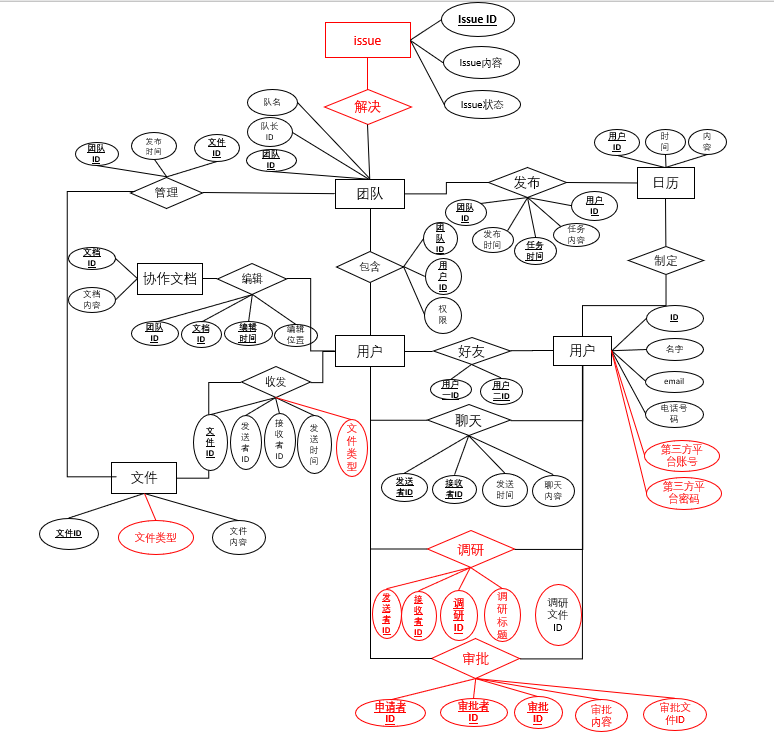
\includegraphics[scale =0.6]{数据库.png}\label{tab:classification}
            \caption{数据库逻辑图}\label{fig:noted-figure}
        \end{figure}
        \newpage


\section{物理设计}
\subsection{数据库产品}
\begin{itemize}
    \item 采用Oracle数据库和Hbase分布式数据库结合
    \item 采用Oracle集中数据库存储文件,用户信息
    \item 采用分布式数据库Hbase(NoSQL)存储聊天信息,多媒体信息
    \item 集中存储用户信息,文件有利于数据管理,分析,隐私保护
    \item 分布存储有利于系统性能提升,且可避免单点失效导致服务丢失
\end{itemize}


\subsection{实体属性、类型、精度}

\subsubsection{用户数据表设计}
\begin{table}[htbp]
\centering
\caption{用户数据表User设计} \label{tab:client-database}
\begin{tabular}{|c|c|c|c|c|}
    \hline
    字段名 & 类型 & 大小 & 说明 & 备注 \\
    \hline
    id & char & 64 & 用户的唯一标识符 & 主键\\
    \hline
    name & char & 64 & 用户的名字 & · \\
    \hline
    email & char  & 64 & 用户的电子邮箱 & · \\
    \hline
    phone & char & 11 & 用户的联系电话 & · \\
    \hline
\end{tabular}
\note{用户数据表User设计}
\end{table}
%========================================
\newpage
\subsubsection{团队数据表设计}
\begin{table}[htbp]
\centering
\caption{团队数据表Group设计} \label{tab:order-database}
\begin{tabular}{|c|c|c|c|c|}
    \hline
    字段名 & 类型 & 大小 & 说明 & 备注 \\
    \hline
    group\_id & char & 64 & 团队的唯一标识符 & 主键\\
    \hline
    leader\_id & char & 64 & 队长的ID & 外键,来自用户表 \\
    \hline
    name & char & 64 & 团队的名字 & · \\
    \hline
\end{tabular}
\note{团队数据表Group设计}
\end{table}
%========================================
\subsubsection{日历数据表设计}
\begin{table}[htbp]
\centering
\caption{日历数据表Calendar设计} \label{tab:order-database}
\begin{tabular}{|c|c|c|c|c|}
    \hline
    字段名 & 类型 & 大小 & 说明 & 备注 \\
    \hline
    id & char & 64 & 日历的唯一标识符 & 主键\\
    \hline
    time & time & 4 & 日历中任务的时间 & · \\
    \hline
    task & char & 512 & 日历中任务的内容 & · \\
    \hline
\end{tabular}
\note{日历数据表Calendar设计}
\end{table}
%========================================
\subsubsection{文件数据表设计}
\begin{table}[htbp]
\centering
\caption{文件数据表File设计} \label{tab:order-database}
\begin{tabular}{|c|c|c|c|c|}
    \hline
    字段名 & 类型 & 大小 & 说明 & 备注 \\
    \hline
    id & char & 64 & 文件的唯一标识符 & 主键\\
    \hline
    file & char & 10G & 文件的内容 & · \\
    \hline
\end{tabular}
\note{文件数据表File设计}
\end{table}
\newpage
%========================================
\subsubsection{协作文档数据表设计}
\begin{table}[htbp]
\centering
\caption{协作文档数据表Coop设计} \label{tab:order-database}
\begin{tabular}{|c|c|c|c|c|}
    \hline
    字段名 & 类型 & 大小 & 说明 & 备注 \\
    \hline
    id & char & 64 & 文档的唯一标识符 & 主键\\
    \hline
    doc & char & 10G & 在线协作文档的内容 & · \\
    \hline
\end{tabular}
\note{协作文档数据表Coop设计}
\end{table}
%========================================
\subsubsection{团队-用户关系数据表设计}
\begin{table}[htbp]
\centering
\caption{包含关系数据表Group\_User} \label{tab:order-database}
\begin{tabular}{|c|c|c|c|c|}
    \hline
    字段名 & 类型 & 大小 & 说明 & 备注 \\
    \hline
    group\_id & char & 64 & 包含关系的标识符之一 & 主键|外键,来自团队表
    \\
    \hline
    user\_id & char & 64 & 包含关系的标识符之一 & 主键|外键,来自用户表 \\
    \hline
    name & char & 64 & 团队的名字 & · \\
    \hline
\end{tabular}
\note{团队-用户包含关系数据表Group\_User设计}
\end{table}
%========================================
\subsubsection{团队-日历关系数据表设计}
\begin{table}[htbp]
\centering
\caption{发布关系数据表Group\_Calendar} \label{tab:order-database}
\begin{tabular}{|c|c|c|c|c|}
    \hline
    字段名 & 类型 & 大小 & 说明 & 备注 \\
    \hline
    group\_id & char & 64 & 发布关系的标识符之一 & 主键|外键,来自团队表
    \\
    \hline
    user\_id & char & 64 & 发布关系的标识符之一 & 主键|外键,来自用户表
    \\
    \hline
    task\_time & time & 4 & 发布关系的标识符之一 & 主键\\
    \hline
    issue\_time & time & 4 & 发布任务的时间 & · \\
    \hline
    task & char & 512 & 发布任务的内容 & · \\  
    \hline
\end{tabular}
\note{团队-日历发布关系数据表Group\_Calendar设计}
\end{table}
\newpage
%========================================
\subsubsection{团队-文件关系数据表设计}
\begin{table}[htbp]
\centering
\caption{管理关系数据表Group\_File} \label{tab:order-database}
\begin{tabular}{|c|c|c|c|c|}
    \hline
    字段名 & 类型 & 大小 & 说明 & 备注 \\
    \hline
    group\_id & char & 64 & 管理关系的标识符之一 & 主键|外键,来自团队表
    \\
    \hline
    file\_id & char & 64 & 管理关系的标识符之一 & 主键|外键,来自文件表
    \\
    \hline
    time & time & 4 & 发布文件的时间 & · \\ 
    \hline
\end{tabular}
\note{团队-文件管理关系数据表Group\_File设计}
\end{table}
%========================================
\subsubsection{用户-协作文档关系数据表设计}
\begin{table}[htbp]
\centering
\caption{编辑关系数据表User\_Coop} \label{tab:order-database}
\begin{tabular}{|c|c|c|c|c|}
    \hline
    字段名 & 类型 & 大小 & 说明 & 备注 \\
    \hline
    user\_id & char & 64 & 编辑关系的标识符之一 & 主键|外键,来自用户表
    \\
    \hline
    file\_id & char & 64 & 编辑关系的标识符之一 & 主键|外键,来自协作文档表 \\
    \hline
    edit\_time & time & 4 & 编辑关系的标识符之一 & 主键 \\ 
    \hline
    edit\_pos & int & 4 & 编辑的位置 & · \\ 
    \hline
\end{tabular}
\note{用户-协作文档编辑关系数据表User\_Coop设计}
\end{table}
\newpage
%========================================
\subsubsection{用户-用户关系数据表设计}
\begin{table}[htbp]
\centering
\caption{好友关系数据表User\_User\_Friend} \label{tab:order-database}
\begin{tabular}{|c|c|c|c|c|}
    \hline
    字段名 & 类型 & 大小 & 说明 & 备注 \\
    \hline
    id1 & char & 64 & 好友关系的标识符之一 & 主键|外键,来自用户表 \\
    \hline
    id2 & char & 64 & 好友关系的标识符之一 & 主键|外键,来自用户表 \\
    \hline
\end{tabular}
\note{好友关系数据表User\_User\_Friend设计}
\end{table}

\begin{table}[htbp]
\centering
\caption{聊天关系数据表User\_User\_Chat} \label{tab:order-database}
\begin{tabular}{|c|c|c|c|c|}
    \hline
    字段名 & 类型 & 大小 & 说明 & 备注 \\
    \hline
    send\_id & char & 64 & 聊天关系的标识符之一 & 主键|外键,来自用户表 \\
    \hline
    recv\_id & char & 64 & 聊天关系的标识符之一 & 主键|外键,来自用户表 \\
    \hline
    time & time & 4 & 聊天信息的发送时间 & · \\ 
    \hline
    message & char & 512 & 聊天内容 & · \\ 
    \hline
\end{tabular}
\note{聊天关系数据表User\_User\_Chat设计}
\end{table}
%========================================
\subsubsection{用户-文件关系数据表设计}
\begin{table}[htbp]
\centering
\caption{收发关系数据表User\_File} \label{tab:order-database}
\begin{tabular}{|c|c|c|c|c|}
    \hline
    字段名 & 类型 & 大小 & 说明 & 备注 \\
    \hline
    send\_id & char & 64 & 收发关系的标识符之一 & 主键|外键,来自用户表 \\
    \hline
    recv\_id & char & 64 & 收发关系的标识符之一 & 主键|外键,来自用户表 \\
    \hline
    file\_id & char & 64 & 收发关系的标识符之一 & 主键|外键,来自文件表 \\
    \hline
    time & time & 4 & 文件的发送时间 & · \\ 
    \hline
\end{tabular}
\note{用户-文件收发关系数据表User\_File设计}
\end{table}



\newpage

\section{安全性设计}
安全性设计主要包括容灾和备份设计。容灾是为了在遭遇灾害时能保证信息系统能正常运行,从而实现业务连续性;备份是为了应对灾难来临时造成的数据丢失问题。

对于即时通讯系统,由于其用户群体巨大且即时通讯需求强,因此遭遇灾害时迅速恢复是至关重要的设计;此外对于用户尤其是企业级用户,文件及数据的机密性,可靠性,可用性等必须通过备份保证。

\subsection{备份设计}
\begin{itemize}
\item 按空间分类,分别进行同城和异地备份。\\
同城备份将数据备份在本地,其特点是速度相对较快。缺点是一旦发生大灾大难,将无法保证本地数据仍可用。 \\

异地备份将数据备份到异地。例如,不能在同一地震带,不能在同地电网,不能在同一江河流域。

\item 按时间分类,每天,每周进行不同级别的备份。\\
1. 每周对数据库进行一次完全备份。\\
2. 每天夜里2:00 am -3:00 am 对数据库的事务日志进行差异备份。\\
3. 在异地建立一个热备份点,通过网络进行同步数据备份。也就是通过网络以同步方式,把主站点的数据备份到备份站点,备份站点一般只备份数据,不承担业务。当出现灾难时,备份站点接替主站点的业务,从而维护业务运行的连续性。\\
\end{itemize}

\subsection{容灾设计}
容灾系统可以分为数据容灾和应用容灾,其实现如下:
\begin{itemize}
     
\item 数据容灾要求建立一个异地的数据系统,在本地数据及整个应用系统出现灾难时,系统至少在异地保存有一份可用的关键业务的数据。

\item 应用容灾要求在异地建立一套完整的与本地生产系统相当的备份应用系统,在灾难情况下,远程系统迅速接管业务运行。其不仅需要一份可用的数据复制,还要有包括网络、主机、应用等资源。主要的技术包括负载均衡、集群技术。

\item 需要高可靠性软件协调应用的切换 \\
高可靠性软件用于自动检测系统的运行状态,在一台服务器出现故障的情况下,自动地把设定的服务转到另一台服务器上。当运行服务器提供的服务不可用时,备份服务器自动接替运行服务器的工作而不用重新启动系统,而当运行服务器恢复正常后,按照使用者的设定以自动或手动方式将服务切换到运行服务上运行。
\end{itemize}

\subsection{权限管理}
为了保证数据的安全,包括其机密性,完整性,可用性,数据库需要对用户进行访问控制。权限管理采用PMI和PKI模型。\\
PMI以资源管理为核心,对资源的访问控制权交由授权机构统一处理,即由资源的所有者来进行访问控制 。PKI以公开密钥技术为基础,以数据的机密性、完整性和无可抵赖性为安全目的而构建的认证、授权、加密等硬件、软件的综合设施


\section{数据库管理与维护说明}
对于数据库的维护,随时对数据库中的信息加以调试和保存备份。同样需要个工作人员进行系统的分析和用户的反馈,对系统进行升级以及功能的完善。同时保证系统安全有序的运行。
\chapter{界面设计}
%==============================================================
    \section{客户端界面}
    \begin{figure}[h]
        \centering
        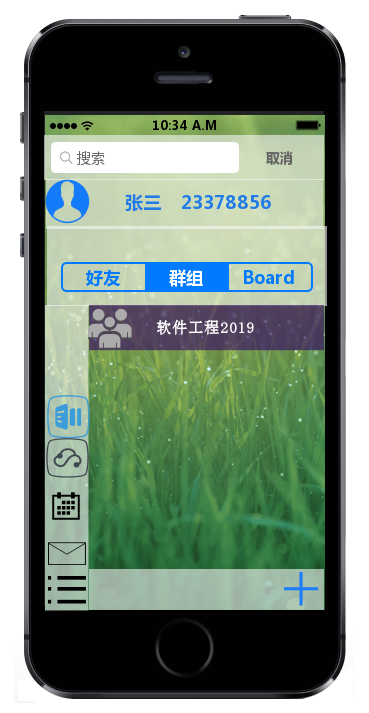
\includegraphics[scale=0.6]{OutlineDesign/figures/客户端界面.png}
        \caption{客户端界面}
        \label{fig:server_flow}
        \note{左下快捷方式从上到下依次为:在线文档协作,云文件管理,日历,邮箱,菜单栏,右下为添加新的好友/群聊}
    \end{figure}
    \newpage
    %--------------------------------------------------------------------------
    \section{服务器端界面}
    %=================================
    % 此处应当有一个简略的图。
    %=================================
    \begin{figure}[h]
        \centering
        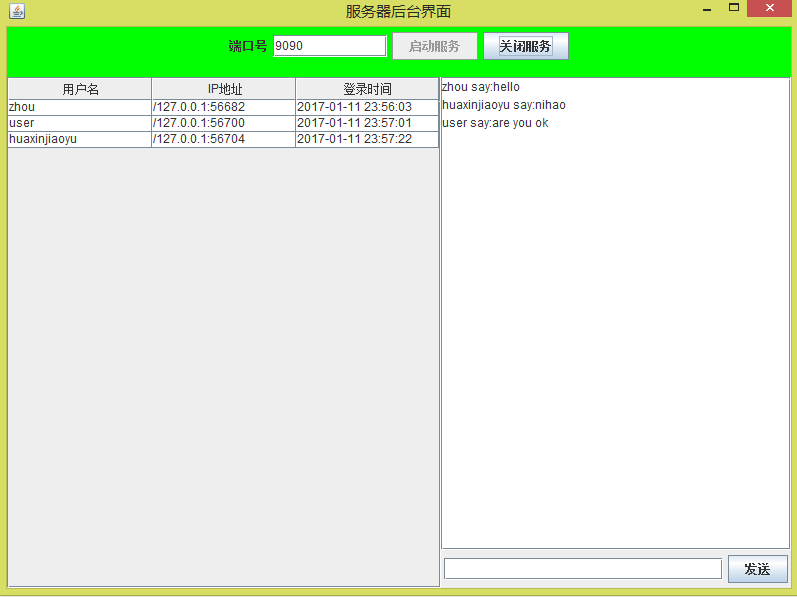
\includegraphics[scale=0.7]{OutlineDesign/figures/服务器端界面.png}
        \caption{服务器端界面}
        \label{fig:server_flow}
    \end{figure}
    \newpage
    %--------------------------------------------------------------------------
    \section{登录界面}
    %=================================
    % 此处应当有一个简略的图。
    %=================================
    \begin{figure}[h]
        \centering
        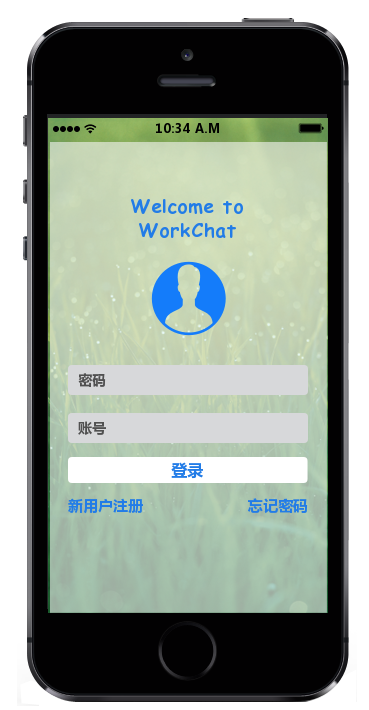
\includegraphics[scale=0.7]{OutlineDesign/figures/登录界面.png}
        \caption{登录界面}
        \label{fig:server_flow}
    \end{figure}
    \newpage
    %--------------------------------------------------------------------------
    \section{R.INTF.CALC.001:一对一即时通讯功能界面}
    %=================================
    % 此处应当有一个简略的图。
    %=================================
    \begin{figure}[h]
        \centering
        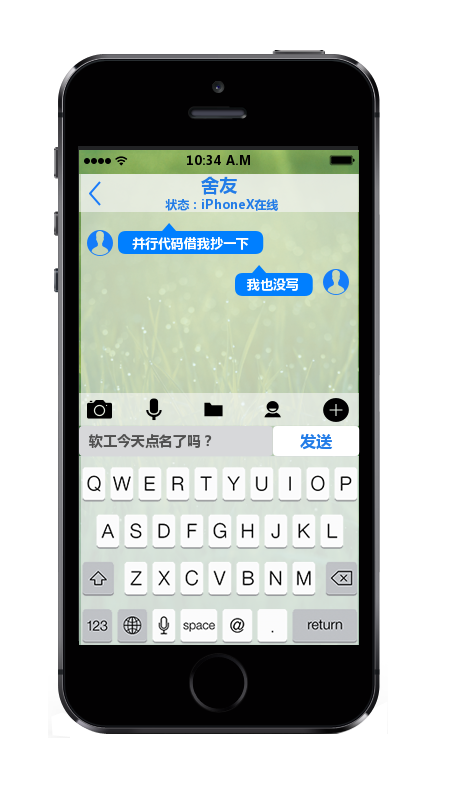
\includegraphics[scale=0.6]{OutlineDesign/figures/一对一即时通讯功能界面.png}
        \caption{一对一即时通讯功能界面}
        \label{fig:server_flow}
    \end{figure}
    \newpage
    %--------------------------------------------------------------------------
    \section{R.INTF.CALC.002.1: 群管理功能界面}
    \begin{figure}[h]
        \centering
        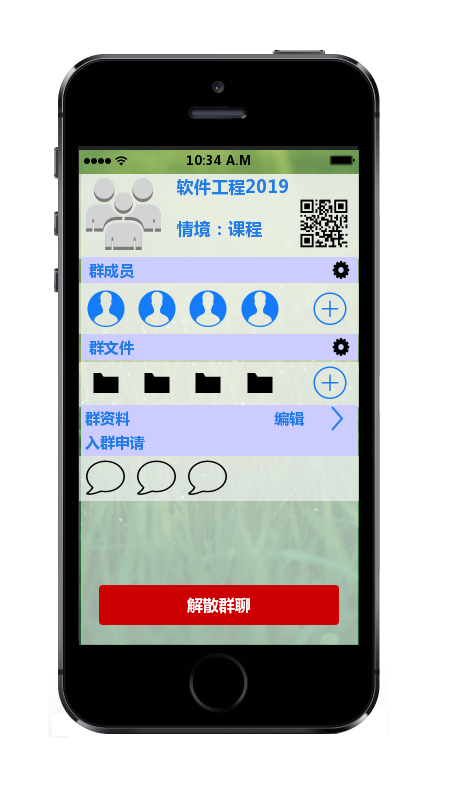
\includegraphics[scale=0.6]{OutlineDesign/figures/群管理功能界面.png}
        \caption{群管理功能界面}
        \label{fig:server_flow}
    \end{figure}
    \newpage
    %--------------------------------------------------------------------------
    \section{R.INTF.CALC.002.2: 群聊天功能界面}
    \begin{figure}[h]
        \centering
        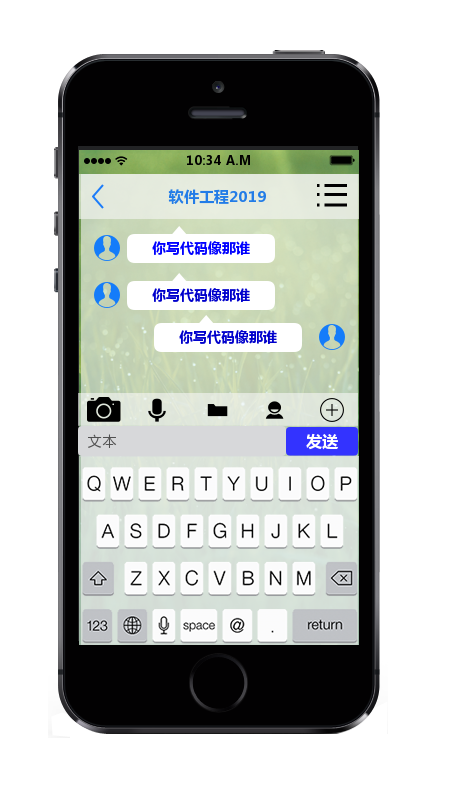
\includegraphics[scale=0.6]{OutlineDesign/figures/群聊天功能界面.png}
        \caption{群聊天功能界面}
        \label{fig:server_flow}
    \end{figure}
    \newpage
    %--------------------------------------------------------------------------
    \section{R.INTF.CALC.002.3: 情境功能界面}
    \begin{figure}[h]
        \centering
        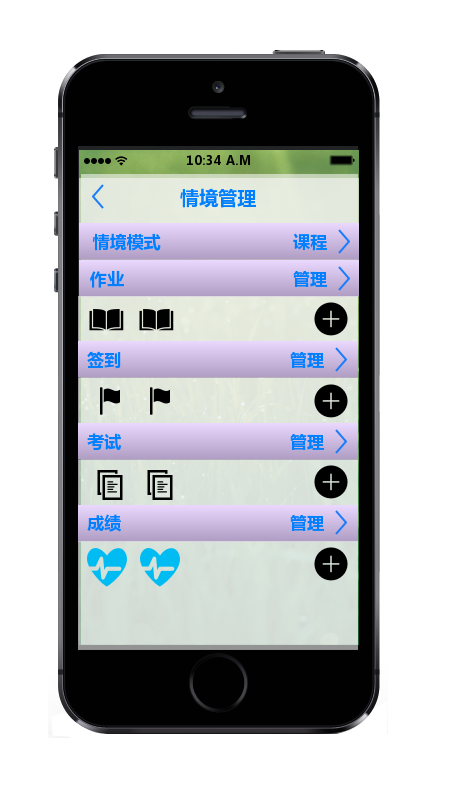
\includegraphics[scale=0.6]{OutlineDesign/figures/情境功能界面.png}
        \caption{情境功能界面}
        \label{fig:server_flow}
    \end{figure}
    \newpage
    %--------------------------------------------------------------------------
    \section{\color{red}R.INTF.CALC.002.4: 问题功能}
    \begin{figure}[h]
        \centering
        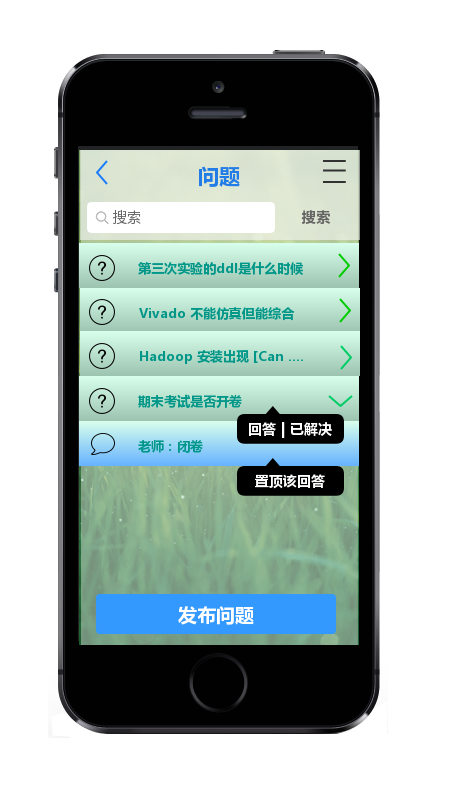
\includegraphics[scale=0.6]{OutlineDesign/figures/问题功能功能界面.png}
        \caption{\color{red}问题功能功能界面}
        \label{fig:server_flow}
    \end{figure}
    \newpage
    %--------------------------------------------------------------------------
    \section{R.INTF.CALC.003: 活动/任务发布与管理功能界面}
    \begin{figure}[h]
        \centering
        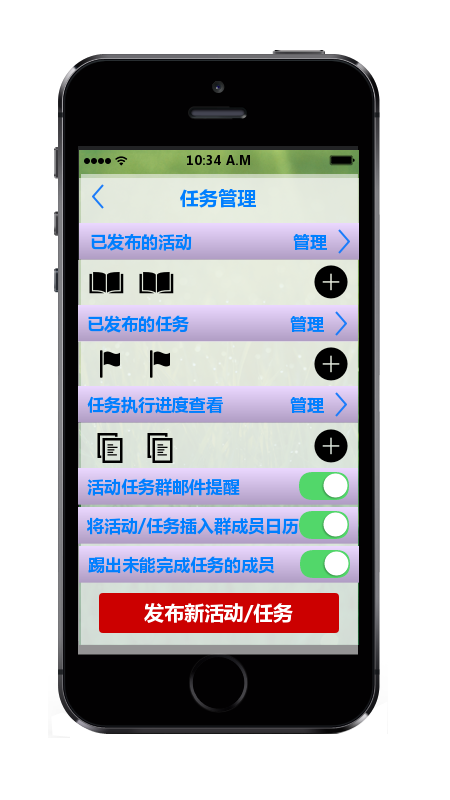
\includegraphics[scale=0.6]{OutlineDesign/figures/活动任务发布与管理功能界面.png}
        \caption{活动任务发布与管理功能界面}
        \label{fig:server_flow}
    \end{figure}
    \newpage
    %--------------------------------------------------------------------------
    \section{R.INTF.CALC.004: 音视频通话 (会议) 功能界面}
    \begin{figure}[h]
        \centering
        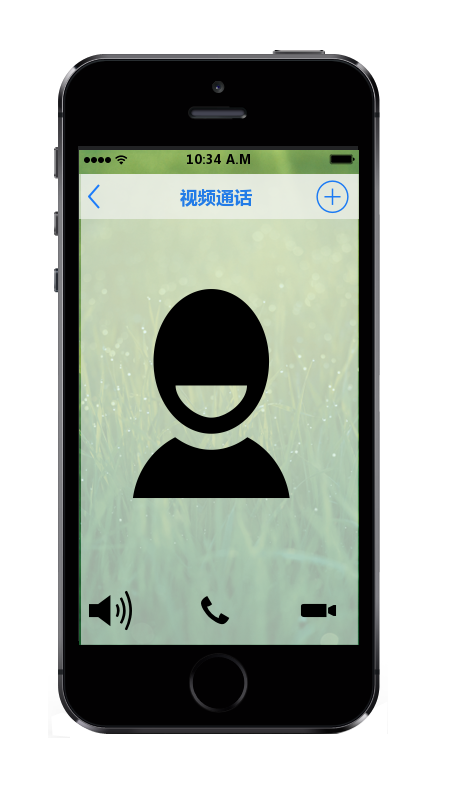
\includegraphics[scale=0.6]{OutlineDesign/figures/音视频通话会议功能界面.png}
        \caption{音视频通话 (会议) 功能界面}
        \label{fig:server_flow}
    \end{figure}
    \newpage
    %--------------------------------------------------------------------------
    \section{R.INTF.CALC.005.1: 好友管理功能界面}
    \begin{figure}[h]
        \centering
        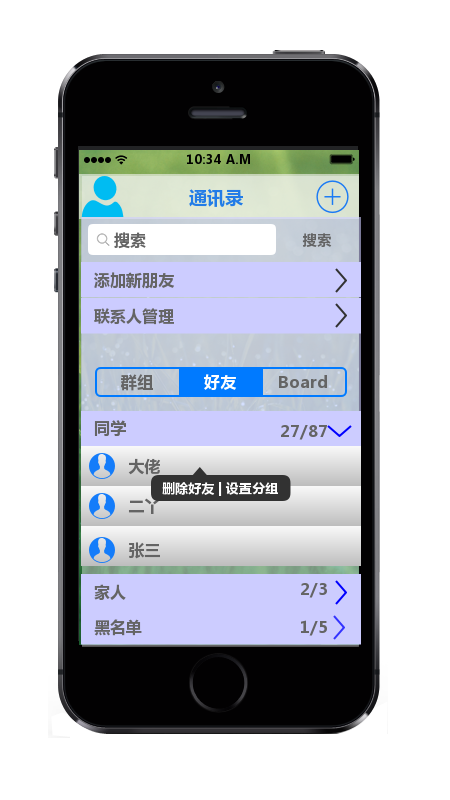
\includegraphics[scale=0.6]{OutlineDesign/figures/好友管理功能界面.png}
        \caption{好友管理功能界面}
        \label{fig:server_flow}
    \end{figure}
    \newpage
    %--------------------------------------------------------------------------
    \section{R.INTF.CALC.005.2: 群聊管理功能界面}
    \begin{figure}[h]
        \centering
        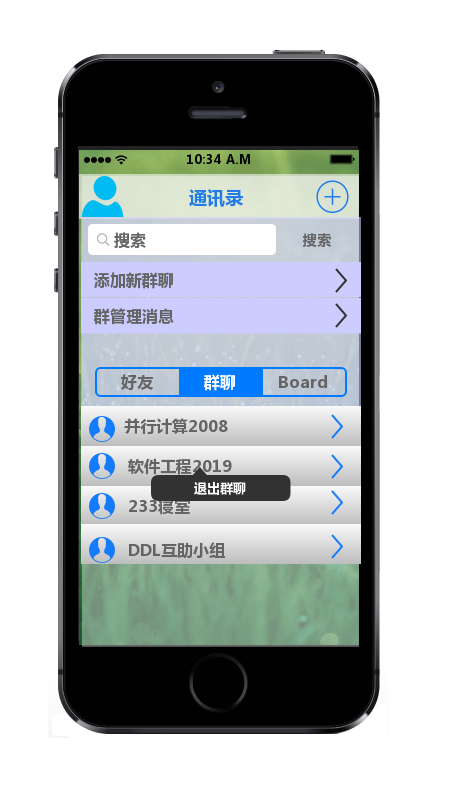
\includegraphics[scale=0.6]{OutlineDesign/figures/群聊管理功能界面.png}
        \caption{群聊管理功能界面}
        \label{fig:server_flow}
    \end{figure}
    \newpage
    %--------------------------------------------------------------------------
    \section{R.INTF.CALC.005.3: 黑名单功能界面}
    \begin{figure}[h]
        \centering
        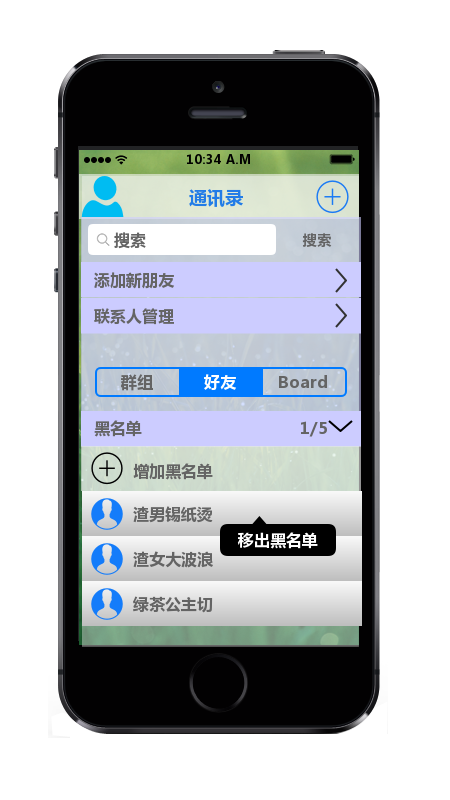
\includegraphics[scale=0.6]{OutlineDesign/figures/黑名单功能界面.png}
        \caption{黑名单功能界面}
        \label{fig:server_flow}
    \end{figure}
    \newpage
    %--------------------------------------------------------------------------
    \section{R.INTF.CALC.006: 聊天记录功能界面}
    \begin{figure}[h]
        \centering
        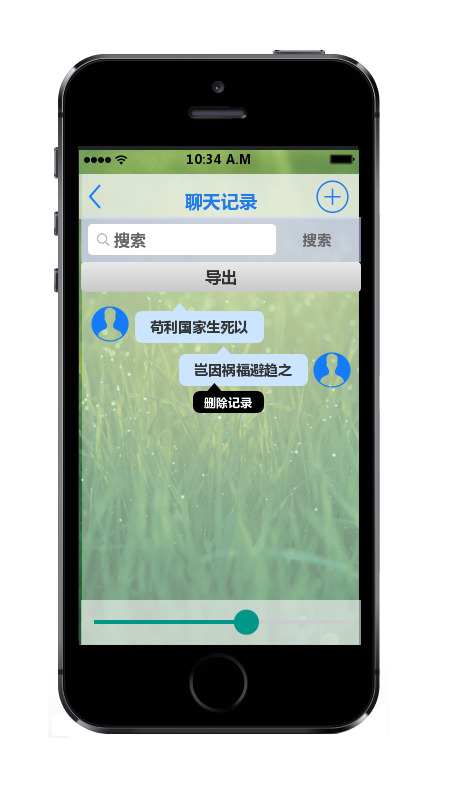
\includegraphics[scale=0.6]{OutlineDesign/figures/聊天记录功能界面.png}
        \caption{聊天记录功能界面}
        \label{fig:server_flow}
    \end{figure}
    \newpage
    %--------------------------------------------------------------------------
    \section{R.INTF.CALC.007: 消息提醒功能界面}
    \begin{figure}[h]
        \centering
        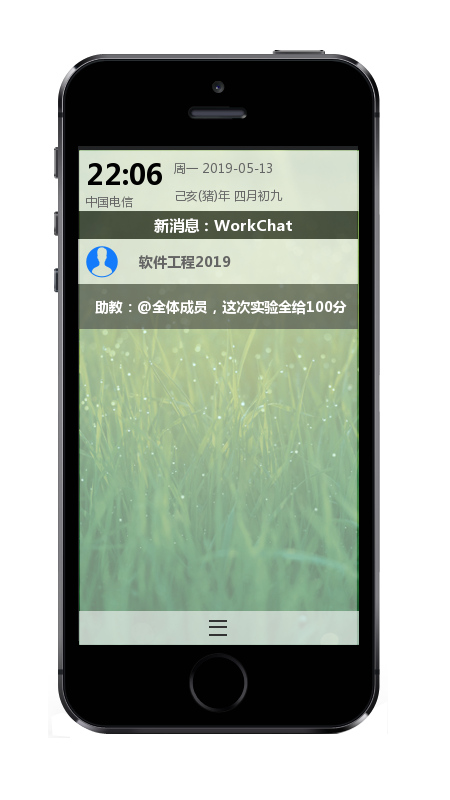
\includegraphics[scale=0.6]{OutlineDesign/figures/消息提醒功能界面.png}
        \caption{消息提醒功能界面}
        \label{fig:server_flow}
    \end{figure}
    \newpage
    %--------------------------------------------------------------------------
    \section{R.INTF.CALC.008: Board(广场) 功能界面}
    \begin{figure}[h]
        \centering
        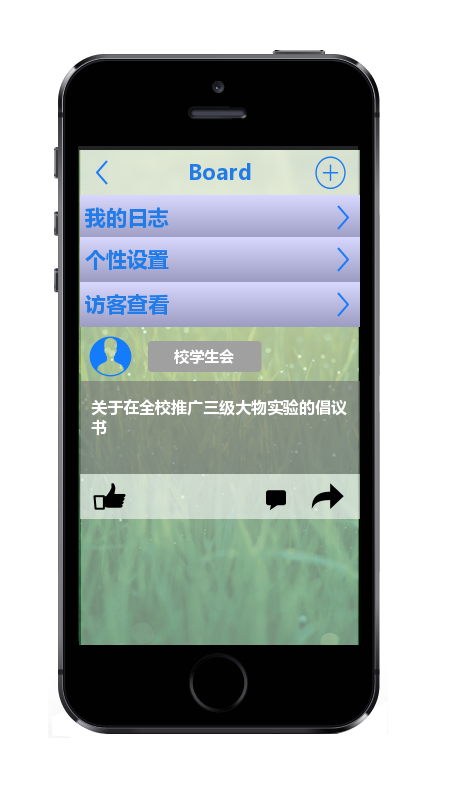
\includegraphics[scale=0.6]{OutlineDesign/figures/Board广场功能界面.png}
        \caption{Board(广场) 功能界面}
        \label{fig:server_flow}
    \end{figure}
    \newpage
    %--------------------------------------------------------------------------
    \section{R.INTF.CALC.009: 个性化好友推荐功能界面}
    \begin{figure}[h]
        \centering
        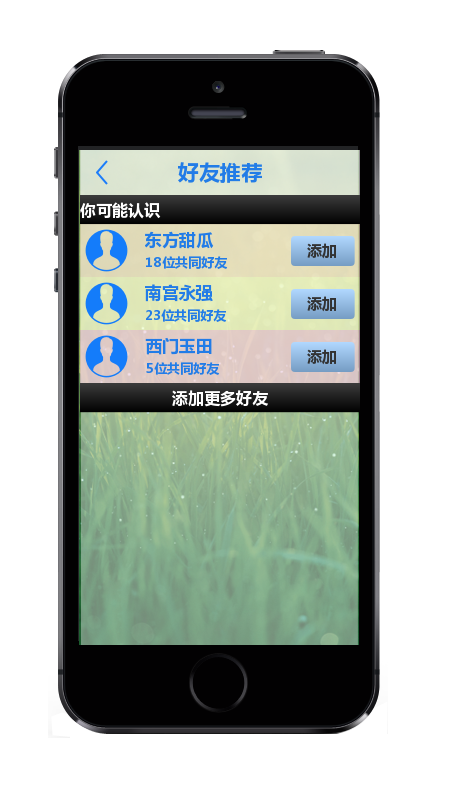
\includegraphics[scale=0.6]{OutlineDesign/figures/个性化好友推荐功能界面.png}
        \caption{个性化好友推荐功能界面}
        \label{fig:server_flow}
    \end{figure}
    \newpage
    %--------------------------------------------------------------------------
    \section{R.INTF.CALC.010: 在线文档协作平台功能界面}
    \begin{figure}[h]
        \centering
        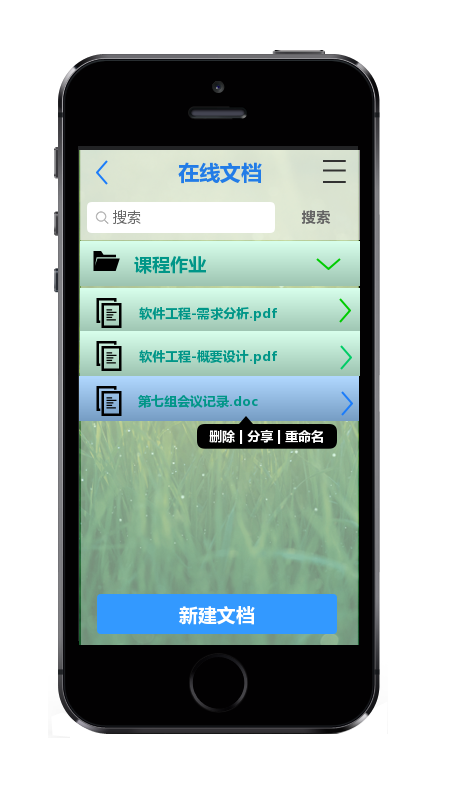
\includegraphics[scale=0.6]{OutlineDesign/figures/在线文档协作平台功能界面.png}
        \caption{在线文档协作平台功能界面}
        \label{fig:server_flow}
    \end{figure}
    \newpage
    %--------------------------------------------------------------------------
    \section{R.INTF.CALC.011: 账号保护和隐私保护功能界面}
    \begin{figure}[h]
        \centering
        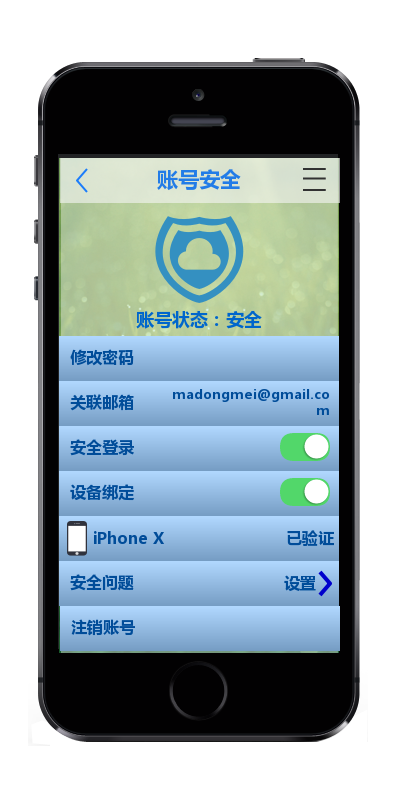
\includegraphics[scale=0.6]{OutlineDesign/figures/账号保护和隐私保护功能界面.png}
        \caption{账号保护和隐私保护功能界面}
        \label{fig:server_flow}
    \end{figure}
    \newpage
    %--------------------------------------------------------------------------
    \section{R.INTF.CALC.012: 日历管理功能界面}
    \begin{figure}[h]
        \centering
        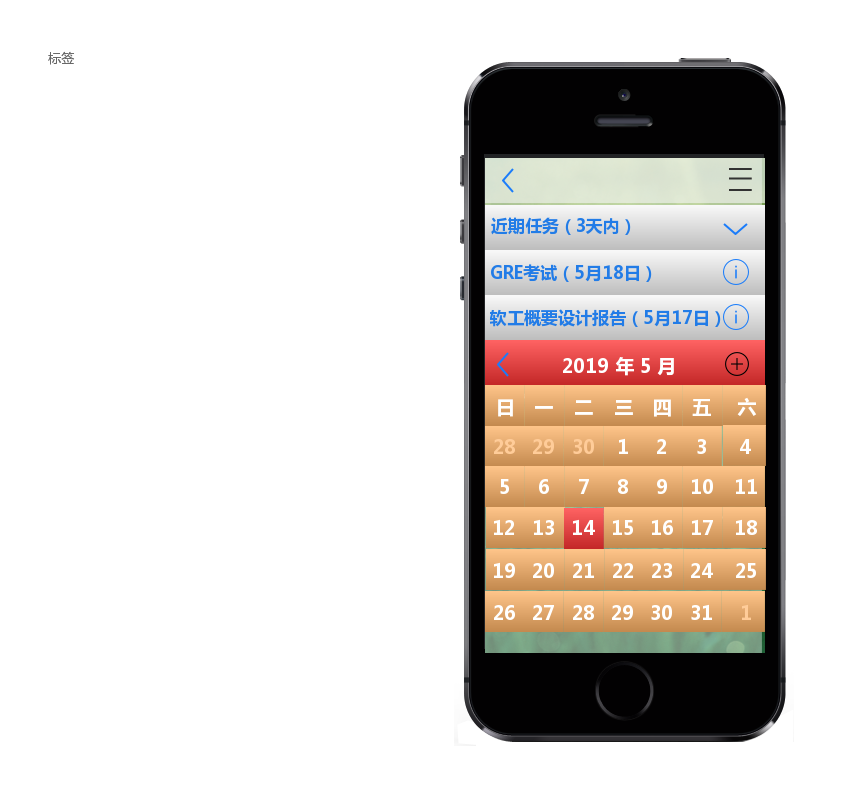
\includegraphics[scale=0.6]{OutlineDesign/figures/日历管理功能界面.png}
        \caption{日历管理功能界面}
        \label{fig:server_flow}
    \end{figure}
    \newpage
    %--------------------------------------------------------------------------
    \section{R.INTF.CALC.013: 个人本地和云端文件管理功能界面}
    \begin{figure}[h]
        \centering
        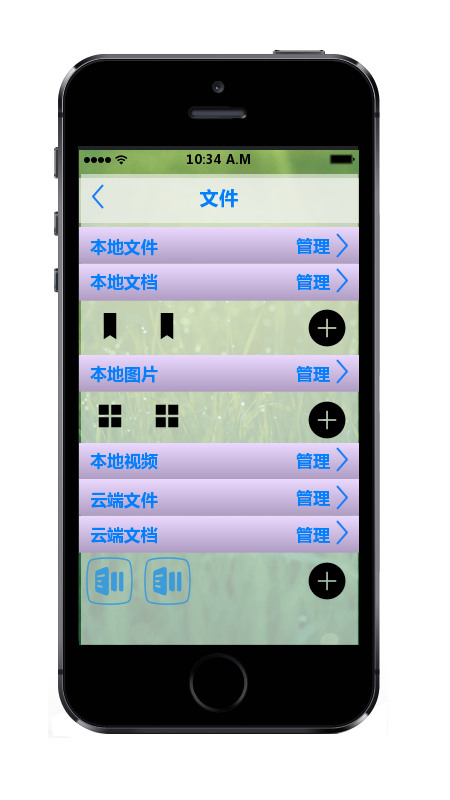
\includegraphics[scale=0.6]{OutlineDesign/figures/个人本地和云端文件管理功能界面.png}
        \caption{个人本地和云端文件管理功能界面}
        \label{fig:server_flow}
    \end{figure}
    \newpage
    %--------------------------------------------------------------------------
    \section{R.INTF.CALC.014: 邮箱接口功能界面}
    \begin{figure}[h]
        \centering
        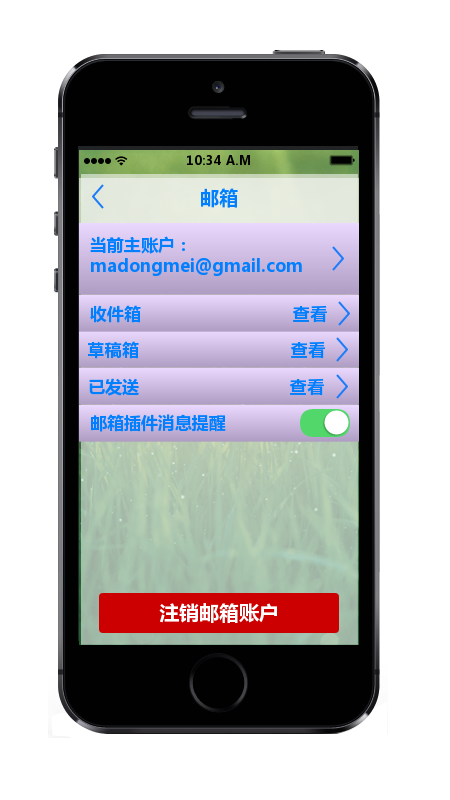
\includegraphics[scale=0.6]{OutlineDesign/figures/邮箱接口功能界面.png}
        \caption{邮箱接口功能界面}
        \label{fig:server_flow}
    \end{figure}
    \newpage
    %--------------------------------------------------------------------------
    \section{\color{red}R.INTF.CALC.015: 流程审批功能}
    \begin{figure}[h]
        \centering
        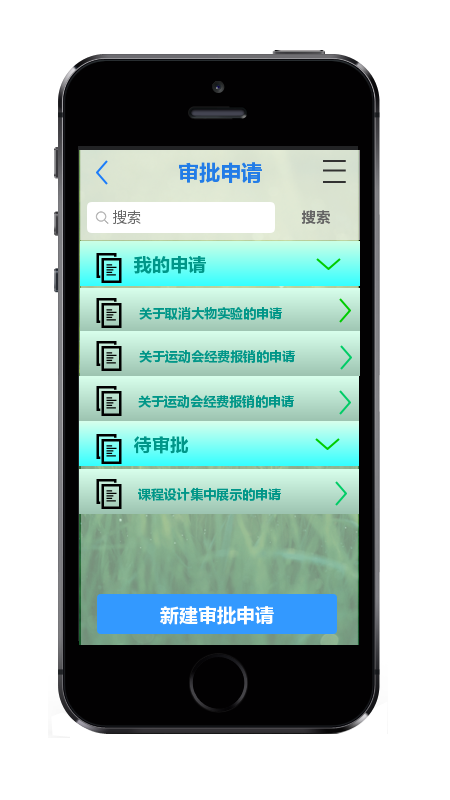
\includegraphics[scale=0.6]{OutlineDesign/figures/流程审批功能界面.png}
        \caption{\color{red}流程审批功能界面}
        \label{fig:server_flow}
    \end{figure}
    \newpage
    %--------------------------------------------------------------------------
    \section{\color{red}R.INTF.CALC.016: 信息调研功能}
    \begin{figure}[h]
        \centering
        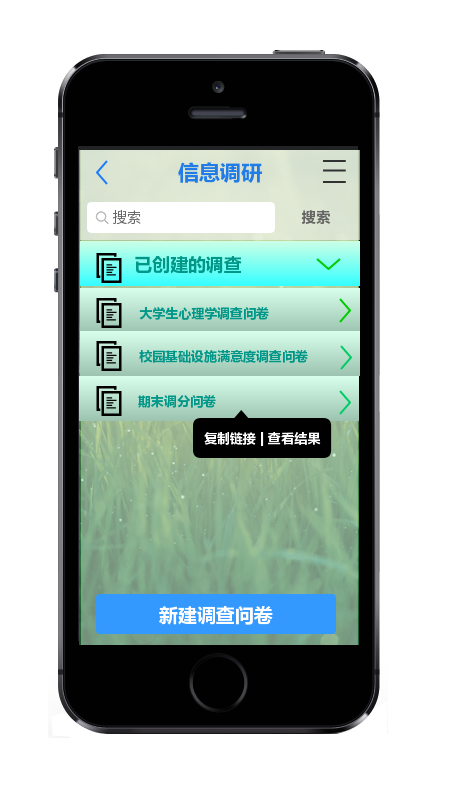
\includegraphics[scale=0.6]{OutlineDesign/figures/信息调研功能界面.png}
        \caption{\color{red}信息调研功能界面}
        \label{fig:server_flow}
    \end{figure}
    \newpage
    %--------------------------------------------------------------------------
    \section{\color{red}R.INTF.CALC.017: 第三方账号同步功能}
    \begin{figure}[h]
        \centering
        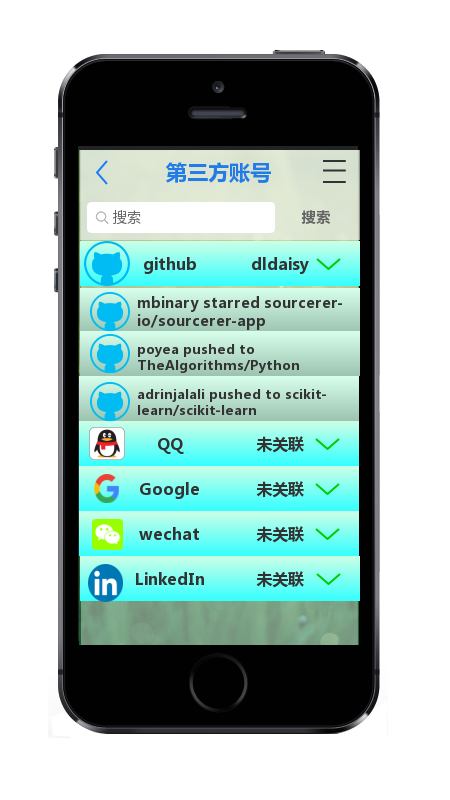
\includegraphics[scale=0.6]{OutlineDesign/figures/第三方账号同步功能界面.png}
        \caption{\color{red}第三方账号同步功能界面}
        \label{fig:server_flow}
    \end{figure}
    \newpage
    %--------------------------------------------------------------------------
    
\chapter{出错处理设计}
\section{数据库出错处理}
多重备份时,应采取何种策略,先利用哪一份备份;系统是否暂停服务等。

\begin{itemize}
    \item 当用户信息数据库出错时,立即启动同步备份的数据库,并将其复制到本地。若依然无法恢复,暂停整个用户系统的服务,向客户端的相关操作返回报错信息。同时派专员进行后台修复和安全性检查。向错误信息处理模块发送错误信息。
    \item  当聊天信息数据库出错时,将数据库回退到上一时间,并根据日志重新向用户发送聊天信息。若无法回退或日志丢失,则调用备份数据库,并向用户返回消息发送失败的信息。对于音视频信息,尝试重新连接。同时派专员进行后台修复和网络检查。向错误信息处理模块发送错误信息。
    \item 当文件或云文件数据库出错时,立即启动同步备份的数据库,并将其复制到本地。若依然无法恢复,向用户返回文件丢失的信息。同时派专员后台排查恶意攻击和隐私泄露的情况。向错误信息处理模块发送错误信息。
    \item 当协作文档数据库出错时,将数据库回退到上一时间,并将缓冲池中的数据写回。若无法回退,则调用其他备份数据库。同时派专员进行后台修复和存储检查。向错误信息处理模块发送错误信息。

\end{itemize}


\section{某模块失效处理}
\subsection{用户信息管理模块失效}
若用户信息管理模块失效,则所有操作均无法正常进行。因此,需要对该服务进行多处热备份。失效时向错误信息管理模块发送错误信息,并立即启用备份服务。后台派专员进行错误检查和恢复。若依然无法继续服务,则整个系统暂停服务。
\subsection{通讯管理模块失效}
若通讯管理模块失效,则聊天,邮件,查询聊天记录等功能无法进行。首先检查是否为网络问题,若是,则切换网络并重启。否则,启用备份服务,发送错误信息,等待后台维护人员处理。若依然失效,则向用户聊天窗口,邮件窗口报错,尽快恢复服务。
\subsection{文件管理模块失效}
若文件管理模块失效,则文件上传,下载,收发,日历功能和部分群组功能会受到影响。失效时首先缓存正在处理的文件,向错误信息管理模块发送错误信息,然后启用备份服务,从而尽快恢复服务。
\subsection{云文件管理模块失效}
若云文件管理模块失效,则部分云文件上传,下载,收发功能会受到影响。失效时依然维持其他服务状态,检查具体失效的功能,暂时禁用失效的部分功能。向错误信息管理模块发送错误信息,后台派专员进行错误检查和恢复。
\subsection{日历管理模块失效}
若日历管理模块失效,则日历的修改,团队任务布置等功能受到影响。失效时暂时禁用日历功能,维持其它功能运行。向错误信息管理模块发送错误信息,后台派专员进行错误检查和恢复。
\subsection{团队管理模块失效}
若团队管理模块失效,则团队信息管理,权限管理,协作文档等功能受到影响。失效时维持最小服务状态(即时通讯),向错误信息管理模块发送错误信息,后台派专员进行错误检查和恢复。
\subsection{在线协作平台模块失效}
若在线协作平台模块失效,则在线协作功能受到影响。失效时,首先缓存正在处理的文档,维持其它功能的运行,禁用团队布置文档和用户编辑文档。向错误信息管理模块发送错误信息,后台派专员进行错误检查和恢复。
\subsection{错误信息管理模块失效}
若错误信息管理模块失效,则各个功能部件传输的错误信息可能无法收到,运维人员发布的错误解决方案可能也无法部署。此时,维持系统正在运行的服务,后台派专员进行错误检查和恢复。

\chapter{\color{red} 安全保密设计}
%===================================================================
% 可能的内容包括保密性、是否采取加密传输、密钥如何分发和管理等。
%===================================================================
    \section{\color{red} 保密性}
    对以下信息在客户端和服务器加密保存,单次使用后立即销毁解密副本:
    \begin{itemize}
        \item 用户信息文件
        \item 用户登录、注册、注销、密码修改信息
        \item 用户安全问题与相关设置信息
        \item 用户操作日志
        \item 用户日历
        \item 用户通讯录
        \item 用户聊天记录
        \item 用户Board日志
        \item 在线文档
        \item 用户邮件
        \item 审批记录
        \item 审批材料
    \end{itemize}
%===================================================================
    \section{加密传输}
    \subsection{RSA算法加密小型数据}
    对客户端和服务器、客户端和客户端之间的小型数据传输,适合采用RSA加密。\\
    例如: 用户名,密码, 验证信息,保密问题等\\
    RSA算法的流程为:
\begin{itemize}
    

 \item 公钥与私钥的产生 \\

1. 选择两个大素数$ {\displaystyle p}$和$ {\displaystyle {q}}$, ${\displaystyle{p}}$ 不等于 ${\displaystyle {q}}$,计算 ${\displaystyle {N=pq}}$。\\
2. 根据欧拉函数,求得$ {\displaystyle r=\varphi (N)=\varphi (p)\varphi (q)=(p-1)(q-1)} $, e与r互质\\
3. 选择一个小于$ {\displaystyle r} $的整数$ {\displaystyle e} $,使 ${\displaystyle e} $与 ${\displaystyle r}$ 互质。\\
4. 并求 ${\displaystyle d} $使得$ {\displaystyle ed\equiv 1{\pmod {r}}}$ 。\\
5. ${\displaystyle (N,e)}$是公钥,${\displaystyle (N,d)}$是私钥。

\item 加密消息\\
加密过程为:\\
${\displaystyle c\equiv n^{e}{\pmod {N}}}$

\item 解密消息 \\
${\displaystyle n\equiv c^{d}\ (\mathrm {mod} \ N)} $
    \end{itemize}
    \subsection{DES算法加密文件等大型数据}
    即时通讯系统中,文件,用户信息,在线文档等大型数据适合采用DES加密。
    DES为对称加密算法。
    与RSA加密算法相比,AES加密算法的优点为加解密的速度更快、加密强度最高、且不占用硬件资源。其更适合加密大型数据。其算法主要分为两步:
    \begin{itemize}
\item 1. 初始置换\\
其功能是把输入的64位数据块按位重新组合,并把输出分为L0、R0两部分,每部分各长32位,其置换规则为将输入的第58位换到第一位,第50位换到第2位……依此类推。
\item 2. 逆置换\\
经过16次迭代运算后,得到L16、R16,将此作为输入,进行逆置换,逆置换正好是初始置换的逆运算,由此即得到密文输出。
     \end{itemize}
%===================================================================
    \section{人机认证与安全问题}
    在登录、注册、修改密码、绑定邮箱等敏感操作的界面添加人机认证(图形/短信验证码,手动滑块)并要求用户回答个人信息和安全设置中的安全问题。
%===================================================================
\chapter{维护设计}
可能的内容包括数据库的日常备份、压缩、维护等。

% \chapter{图片}
本章展示图片相关用法。

\section{示例}
\begin{figure}[ht]
\centering

\includegraphics[width=10cm]{ustc_logo_fig}
\caption{测试图片} \label{fig:figure1}
\end{figure}

\section{带图注的图}
\begin{figure}[ht]
\centering

\includegraphics[width=10cm]{ustc_logo_fig}
\caption{带图注的图片}\label{fig:noted-figure}
\note{the solid lines represent the time histogram of the spontaneous activities of an old monkey cell(gray) and a young monkey cell (black). The bin-width is 1}
\end{figure}

% \chapter{表格}

\section{A Simple Table}
\begin{table}[htbp]
\centering
\caption{这里是表的标题} \label{tab:simpletable}
\begin{tabular}{|c|c|}
    \hline
    a & b \\
    \hline
    c & d \\
    \hline
\end{tabular}
\note{这里是表的注释}
\end{table}

\section{长表格}
\begin{longtable}{ccc}
% 首页表头
\caption[长表格演示]{长表格演示} \label{tab:longtable} \\
\toprule[1.5pt]
名称  & 说明 & 备注\\
\midrule[1pt]
\endfirsthead
% 续页表头
\caption[]{长表格演示(续)} \\
\toprule[1.5pt]
名称  & 说明 & 备注 \\
\midrule[1pt]
\endhead
% 首页表尾
\hline
\multicolumn{3}{r}{\small 续下页}
\endfoot
% 续页表尾
\bottomrule[1.5pt]
\endlastfoot

AAAAAAAAAAAA   &   BBBBBBBBBBB   &   CCCCCCCCCCCCCC   \\
AAAAAAAAAAAA   &   BBBBBBBBBBB   &   CCCCCCCCCCCCCC   \\
AAAAAAAAAAAA   &   BBBBBBBBBBB   &   CCCCCCCCCCCCCC   \\
AAAAAAAAAAAA   &   BBBBBBBBBBB   &   CCCCCCCCCCCCCC   \\
AAAAAAAAAAAA   &   BBBBBBBBBBB   &   CCCCCCCCCCCCCC   \\
AAAAAAAAAAAA   &   BBBBBBBBBBB   &   CCCCCCCCCCCCCC   \\
AAAAAAAAAAAA   &   BBBBBBBBBBB   &   CCCCCCCCCCCCCC   \\
AAAAAAAAAAAA   &   BBBBBBBBBBB   &   CCCCCCCCCCCCCC   \\
AAAAAAAAAAAA   &   BBBBBBBBBBB   &   CCCCCCCCCCCCCC   \\
AAAAAAAAAAAA   &   BBBBBBBBBBB   &   CCCCCCCCCCCCCC   \\
AAAAAAAAAAAA   &   BBBBBBBBBBB   &   CCCCCCCCCCCCCC   \\
AAAAAAAAAAAA   &   BBBBBBBBBBB   &   CCCCCCCCCCCCCC   \\
AAAAAAAAAAAA   &   BBBBBBBBBBB   &   CCCCCCCCCCCCCC   \\
AAAAAAAAAAAA   &   BBBBBBBBBBB   &   CCCCCCCCCCCCCC   \\
AAAAAAAAAAAA   &   BBBBBBBBBBB   &   CCCCCCCCCCCCCC   \\
AAAAAAAAAAAA   &   BBBBBBBBBBB   &   CCCCCCCCCCCCCC   \\
AAAAAAAAAAAA   &   BBBBBBBBBBB   &   CCCCCCCCCCCCCC   \\
AAAAAAAAAAAA   &   BBBBBBBBBBB   &   CCCCCCCCCCCCCC   \\
AAAAAAAAAAAA   &   BBBBBBBBBBB   &   CCCCCCCCCCCCCC   \\
AAAAAAAAAAAA   &   BBBBBBBBBBB   &   CCCCCCCCCCCCCC   \\
AAAAAAAAAAAA   &   BBBBBBBBBBB   &   CCCCCCCCCCCCCC   \\
AAAAAAAAAAAA   &   BBBBBBBBBBB   &   CCCCCCCCCCCCCC   \\
AAAAAAAAAAAA   &   BBBBBBBBBBB   &   CCCCCCCCCCCCCC   \\
AAAAAAAAAAAA   &   BBBBBBBBBBB   &   CCCCCCCCCCCCCC   \\
AAAAAAAAAAAA   &   BBBBBBBBBBB   &   CCCCCCCCCCCCCC   \\
AAAAAAAAAAAA   &   BBBBBBBBBBB   &   CCCCCCCCCCCCCC   \\
AAAAAAAAAAAA   &   BBBBBBBBBBB   &   CCCCCCCCCCCCCC   \\
AAAAAAAAAAAA   &   BBBBBBBBBBB   &   CCCCCCCCCCCCCC   \\
AAAAAAAAAAAA   &   BBBBBBBBBBB   &   CCCCCCCCCCCCCC   \\
AAAAAAAAAAAA   &   BBBBBBBBBBB   &   CCCCCCCCCCCCCC   \\
AAAAAAAAAAAA   &   BBBBBBBBBBB   &   CCCCCCCCCCCCCC   \\
AAAAAAAAAAAA   &   BBBBBBBBBBB   &   CCCCCCCCCCCCCC   \\
AAAAAAAAAAAA   &   BBBBBBBBBBB   &   CCCCCCCCCCCCCC   \\
AAAAAAAAAAAA   &   BBBBBBBBBBB   &   CCCCCCCCCCCCCC   \\
AAAAAAAAAAAA   &   BBBBBBBBBBB   &   CCCCCCCCCCCCCC   \\
AAAAAAAAAAAA   &   BBBBBBBBBBB   &   CCCCCCCCCCCCCC   \\
\end{longtable}

% \chapter{算法环境}
模板中使用 \texttt{algorithm2e} 宏包实现算法环境。关于该宏包的具体用法,
请阅读宏包的官方文档。

\begin{algorithm}[htbp]
\SetAlgoLined
\KwData{this text}
\KwResult{how to write algorithm with \LaTeX2e }

initialization\;
\While{not at end of this document}{
    read current\;
    \eIf{understand}{
        go to next section\;
        current section becomes this one\;
    }{
        go back to the beginning of current section\;
    }
}
\caption{算法示例1}
\label{algo:algorithm1}
\end{algorithm}

\IncMargin{1em}
\begin{algorithm}
\SetKwData{Left}{left}\SetKwData{This}{this}\SetKwData{Up}{up}
\SetKwFunction{Union}{Union}\SetKwFunction{FindCompress}{FindCompress}
\SetKwInOut{Input}{input}\SetKwInOut{Output}{output}

\Input{A bitmap $Im$ of size $w\times l$}
\Output{A partition of the bitmap}
\BlankLine
\emph{special treatment of the first line}\;
\For{$i\leftarrow 2$ \KwTo $l$}{
    \emph{special treatment of the first element of line $i$}\;
    \For{$j\leftarrow 2$ \KwTo $w$}{\label{forins}
        \Left$\leftarrow$ \FindCompress{$Im[i,j-1]$}\;
        \Up$\leftarrow$ \FindCompress{$Im[i-1,]$}\;
        \This$\leftarrow$ \FindCompress{$Im[i,j]$}\;
        \If(\tcp*[h]{O(\Left,\This)==1}){\Left compatible with \This}{\label{lt}
            \lIf{\Left $<$ \This}{\Union{\Left,\This}}
            \lElse{\Union{\This,\Left}}
        }
        \If(\tcp*[f]{O(\Up,\This)==1}){\Up compatible with \This}{\label{ut}
        \lIf{\Up $<$ \This}{\Union{\Up,\This}}
        \tcp{\This is put under \Up to keep tree as flat as possible}\label{cmt}
        \lElse{\Union{\This,\Up}}\tcp*[h]{\This linked to \Up}\label{lelse}
        }
    }
    \lForEach{element $e$ of the line $i$}{\FindCompress{p}}
}
\caption{算法示例2}\label{algo_disjdecomp}
\label{alog:algorithm2}
\end{algorithm}\DecMargin{1em}

% \chapter{代码环境}
模板中使用 \texttt{listings} 宏包实现代码环境。详细用法见宏包的官方说明文档。

以下是代码示例,可以在文中任意位置引用\autoref{first-code} 。
\begin{lstlisting}[language=C, caption=示例代码, label={code:first-code}]
#include <stdio.h>

int main( )
{
    printf("hello, world\n");
    return 0;
}
\end{lstlisting}

% \chapter{引用文献标注}

\section{著者-出版年制标注法}

\noindent
\verb|\citestyle{ustcauthoryear}|
\citestyle{ustcauthoryear}

\noindent
\begin{tabular}{l@{\quad$\Rightarrow$\quad}l}
  \verb|\cite{knuth86a}| & \cite{knuth86a}\\
  \verb|\citet{knuth86a}| & \citet{knuth86a}\\
  \verb|\citet[chap.~2]{knuth86a}| & \citet[chap.~2]{knuth86a}\\[0.5ex]
  \verb|\citep{knuth86a}| & \citep{knuth86a}\\
  \verb|\citep[chap.~2]{knuth86a}| & \citep[chap.~2]{knuth86a}\\
  \verb|\citep[see][]{knuth86a}| & \citep[see][]{knuth86a}\\
  \verb|\citep[see][chap.~2]{knuth86a}| & \citep[see][chap.~2]{knuth86a}\\[0.5ex]
  \verb|\citet*{knuth86a}| & \citet*{knuth86a}\\
  \verb|\citep*{knuth86a}| & \citep*{knuth86a}\\
\end{tabular}

\noindent
\begin{tabular}{l@{\quad$\Rightarrow$\quad}l}
  \verb|\citet{knuth86a,tlc2}| & \citet{knuth86a,tlc2}\\
  \verb|\citep{knuth86a,tlc2}| & \citep{knuth86a,tlc2}\\
  \verb|\cite{knuth86a,knuth84}| & \cite{knuth86a,knuth84}\\
  \verb|\citet{knuth86a,knuth84}| & \citet{knuth86a,knuth84}\\
  \verb|\citep{knuth86a,knuth84}| & \citep{knuth86a,knuth84}\\
\end{tabular}

\section{顺序编码制标注法}

\noindent
\verb|\citestyle{ustcnumerical}|
\citestyle{ustcnumerical}

\noindent
\begin{tabular}{l@{\quad$\Rightarrow$\quad}l}
  \verb|\cite{knuth86a}| & \cite{knuth86a}\\
  \verb|\citet{knuth86a}| & \citet{knuth86a}\\
  \verb|\citet[chap.~2]{knuth86a}| & \citet[chap.~2]{knuth86a}\\[0.5ex]
  \verb|\citep{knuth86a}| & \citep{knuth86a}\\
  \verb|\citep[chap.~2]{knuth86a}| & \citep[chap.~2]{knuth86a}\\
  \verb|\citep[see][]{knuth86a}| & \citep[see][]{knuth86a}\\
  \verb|\citep[see][chap.~2]{knuth86a}| & \citep[see][chap.~2]{knuth86a}\\[0.5ex]
  \verb|\citet*{knuth86a}| & \citet*{knuth86a}\\
  \verb|\citep*{knuth86a}| & \citep*{knuth86a}\\
\end{tabular}

\noindent
\begin{tabular}{l@{\quad$\Rightarrow$\quad}l}
  \verb|\citet{knuth86a,tlc2}| & \citet{knuth86a,tlc2}\\
  \verb|\citep{knuth86a,tlc2}| & \citep{knuth86a,tlc2}\\
  \verb|\cite{knuth86a,knuth84}| & \cite{knuth86a,knuth84}\\
  \verb|\citet{knuth86a,knuth84}| & \citet{knuth86a,knuth84}\\
  \verb|\citep{knuth86a,knuth84}| & \citep{knuth86a,knuth84}\\
  \verb|\cite{knuth86a,knuth84,tlc2}| & \cite{knuth86a,knuth84,tlc2}\\
\end{tabular}

\section{其他形式的标注}

\noindent
\begin{tabular}{l@{\quad$\Rightarrow$\quad}l}
  \verb|\citealt{tlc2}| & \citealt{tlc2}\\
  \verb|\citealt*{tlc2}| & \citealt*{tlc2}\\
  \verb|\citealp{tlc2}| & \citealp{tlc2}\\
  \verb|\citealp*{tlc2}| & \citealp*{tlc2}\\
  \verb|\citealp{tlc2,knuth86a}| & \citealp{tlc2,knuth86a}\\
  \verb|\citealp[pg.~32]{tlc2}| & \citealp[pg.~32]{tlc2}\\
  \verb|\citenum{tlc2}| & \citenum{tlc2}\\
  \verb|\citetext{priv.\ comm.}| & \citetext{priv.\ comm.}\\
\end{tabular}

\noindent
\begin{tabular}{l@{\quad$\Rightarrow$\quad}l}
  \verb|\citeauthor{tlc2}| & \citeauthor{tlc2}\\
  \verb|\citeauthor*{tlc2}| & \citeauthor*{tlc2}\\
  \verb|\citeyear{tlc2}| & \citeyear{tlc2}\\
  \verb|\citeyearpar{tlc2}| & \citeyearpar{tlc2}\\
\end{tabular}

\nocite{*}
\bibliography{bib/tex}

\end{document}
